%!TEX root = ../main.tex

\chapter{Hermes}
\label{ch:hermes}

\lhead{Hermes: Efficient Kinetic Analysis of RNA Molecules}

\section{Introduction}
\label{sec:hermes:intro}

In this chapter, we present the \hermes software suite---a collection of
programs aimed at evaluating the kinetic properties of RNA molecules.
Provided a coarse-grained energy landscape generated by \ffttwo (described
in \Chref{ffttwo}), we present software which computes both the \mfpt
and \eqt for this discretized energy landscape. We also provide software which
computes the exact kinetics for an RNA molecule, however since this requires
exhaustive enumeration of all secondary structures---which is known to be an
exponential quantity for the length of the RNA in consideration---the full
kinetics are not expected to be practical for anything beyond a sequence of
trivial length. The software in \hermes presents a practical application of
the energy landscapes computed by the \ffttwo algorithm. Contrasted against
the other kinetics software in the field, \hermes offers similar accuracy
with unparalleled performance which opens up the possibility for large-scale
kinetic analysis {\em in silico}, which we expect to be of use for synthetic
design.

\subsection{Organization}
\label{subsec:hermes:org}

This chapter is organized in the following fashion. We begin by providing
background on the state-of-the-art approaches for kinetic analysis of RNAs.
From there, we move into a technical discussion of two traditional approaches
for kinetics, computation of the \mfpt and the \eqt. With this foundation in
place, we proceed to discuss the high-level organization of the \hermes
software package, and describe in detail each of the four underlying programs
which comprise the kinetics suite. We then move on to present comparitive
benchmarking of \hermes against other methods, before finally concluding with
some remarks on the accuracy and applicability of \hermes to computational
RNA design.

\section{Background}
\label{sec:hermes:bkgrnd}

Remarkable results in RNA synthetic biology have recently been
obtained by various groups. In \citep{hochrein.jacs13}, small
conditional RNAs have been engineered to silence a gene Y by using the
RNA interference machinery, only if a gene X is transcribed. In
\citep{wachsmuth.nar13} a novel theophylline \rb has been
computationally designed to transcriptionally regulate a gene in
{\em E. coli}, and in \citep{synthetichammerheads} a purely computational
approach was used to design functionally active hammerhead ribozymes.
Computational design of synthetic RNA molecules invariably uses some
form of thermodynamics-based algorithm; indeed, \ms{NUPACK-Design}
\citep{zadeh.jcc11} was used to design small conditional RNAs
\citep{hochrein.jacs13}, Vienna RNA Package \citep{gruber08} was used in
the design of the synthetic theophylline \rb, and the
\ms{RNAiFold} inverse folding software
\citep{garcia.jbcbb13,garciamartin.nar13} was used to design the
synthetic hammerhead ribozymes. The next step in the computational
design of synthetic RNA molecules is to control the kinetics of
folding---such control could be important in engineering
conformational switches. Kinetics is already used as a design feature
for synthetic design in proteins \citep{bujotzek.jcam11,fasting.acie12}.

In this chapter we introduce a new software suite, called \hermes
\citep{senter:2015fq},
which efficiently computes RNA secondary structure
folding kinetics by using a coarse-grained
method to model RNA transitions that add or remove a single base pair.
Since our motivation in developing \hermes is to provide a new
tool to aid in engineering synthetic RNA molecules with desired
kinetic properties, \hermes does not model {\em co-transcriptional
folding}, but only the {\em refolding} of RNA sequences.

There is a rich history of both experimental and computational work on
RNA folding pathways and kinetics. Experimental approaches to
determine the kinetics of RNA folding include temperature jump
experiments \citep{lecuyercrothers}, using fluorophores
\citep{hobartner.jmb03}, using mechanical tension at the single
molecule level \citep{vieregg.mp06}, etc. and will not be further
discussed. Computational approaches to folding kinetics commonly model
stepwise transitions between secondary structures,
involving the addition or removal of a single base
pair, as first considered in \citep{flammhofacker}.
Nevertheless, it should be noted that there are a number of
methods that concern the addition or removal of an entire helical
region, e.g. \citep{huang.bb14,zhao.jcp11}.

Most computational approaches involve either
\begin{inparaenum}[\em 1\upshape)]
\item algorithms to determine optimal or near-optimal folding pathways;
\item explicit solutions of the master equation; or
\item repeated simulations to fold an initially empty secondary structure to
the target \mfe (MFE) structure.
\end{inparaenum}
Examples of methods to determine optimal or
near-optimal folding pathways include the greedy approach of Morgan
and Higgs \citep{morganhiggsbarrier}, the exact, optimal, exponential
time program \barriers \citep{flammhofacker}, the program
\ms{Findpath} \citep{flamm.r01}, which uses bounded look-ahead
breadth-first search, a genetic algorithm \citep{shapiro.jmb01}, the
program \ms{RNAtabupath} that uses local search to determine
near-optimal folding pathways, the Basin Hopping Graph
(BHG, \citep{kucharik:2014ft}) which uses a greedy algorithm to determine local minima
and approximate their barrier energies, etc. The program \barriers
\citep{flammhofacker} is the only current method guaranteed to
produce optimal folding pathways. Since it has been shown that
the problem of determining optimal folding pathways is
NP-complete \citep{thachuk.psb10}, it is now understandable why
\ms{barriers} can take exponential time to converge, depending
on the RNA sequence. For this reason, near-optimal solutions
provided by heuristic methods, such as \ms{RNAtabupath}, are very useful.

Methods that employ the master equation include \ms{Treekin}
\citep{wolfingerstadler:kinetics}, which uses the programs
\ms{RNAsubopt} \citep{wuchtyfontanahofackerschuster} and \barriers
\citep{flammhofacker} to determine {\em macrostates}, defined as basins
of attraction near a locally optimal structure. The resulting
coarse-grained Markov chain is then sufficiently small to allow explicit
solution of the master equation. In \citep{tang.jcb05}, a moderate
number of RNA structures were sampled according to different
strategies, from which a robotic motion planning graph was defined
to connect each sampled structure to its $k$ nearest sampled
neighbors. Again, the resulting coarse-grained Markov chain is
sufficiently small for an explicit solution of the master equation to
be given.

We now come to simulation approaches to estimate RNA folding kinetics.
The program \kinfold \citep{flammphd,flamm} is an implementation
of Gillespie's algorithm \citep{gillespiestochasticsimulation1},
directly related to the master equation, hence is considered by many
to be the {\em gold standard} for RNA kinetics. A recent extension of the
\kinfold algorithm was reported in \citep{aviram.amb12}.
\ms{KFOLD} \citep{dykeman:2015bxa} also implements Gillespie's algorithm,
but leverages memoization of transition rates to operate much more efficiently
than \kinfold. Meanwhile \ms{Kinefold} \citep{xayaphoummine.nar05} uses
stochastic simulations of
the nucleation and dissociation of helical regions to predict
secondary structure and folding pathways. In contrast to the
previously mentioned methods, both \ms{RNAKinetics}
\citep{danilova.jbcb06} and \ms{Kinwalker} \citep{geis.jmb08} model
co-transcriptional folding, known to be necessary when simulating
{\em in vivo} folding of long RNA molecules \citep{lai.r13}. As well,
\ms{Kinefold} can simulate both refolding and co-transcriptional folding
pathways. Finally, unlike all the previous simulation results, which
depend on thermodynamic free energy parameters \citep{turner.nar10},
the program \ms{Oxfold} \citep{anderson.b13} performs kinetic folding
of RNA using stochastic context-free grammars and evolutionary
information.

In contrast to the previous methods, \hermes computes the \mfpt (MFPT)
and \eqt for a
coarse-grained Markov chain consisting of the ensemble of all
secondary structures having \bpd $x$ [resp. $y$] from
reference structures \strA [resp. \strBresp] of a given RNA sequence.
\Mfpt (MFPT) is computed exactly by matrix inversion,
and equilibrium time is computed using spectral decomposition of the rate
matrix for the coarse-grained master equation.

\section{Traditional approaches for kinetics}
\label{sec:hermes:kinetics}

To better understand the underlying algorithms behind the software,
we describe two traditional approaches in kinetics, \mfpt and \eqt.

\subsection{\Mfpt}
\label{subsec:hermes:mfpt}

Consider a physical process,
which when monitored over time, yields the stochastic sequence
$q_0,q_1,q_2,\dots$ of discrete, observed states. If the transition from
state $q_t$ to $q_{t+1}$ depends only on $q_t$ at time
$t$ and not on the historical sequence of prior states visited,
as often assumed in the case of protein or
RNA folding, then a Markov chain provides a reasonable
mathematical model to simulate the process.

A first-order, time-homogeneous
{\em Markov chain} $\mChain = (Q,\pi,P)$ is given by a finite
set $Q = \{ 1,\dots,n \}$ of states, an initial probability distribution
$\pi = (\pi_1,\dots,\pi_n)$, and the $n \times n$
{\em transition probability matrix} $P = (p_{i,j})$.
At time $t=0$, the initial state of the system is
$q_t=i$ with probability $\pi_i$, and at discrete time
$t=1,2,3,\dots$, the system makes a transition from state
$i$ to state $j$ with probability $p_{i,j}$; i.e.
the conditional probability $Pr[ q_{t+1} = j | q_t=i] = p_{i,j}$.
Define the {\em population occupancy frequency} of visiting state
$i$ at time $t$ by $p_{i}(t) = Pr[q_t=i]$.  Denote
$p_{i,j}^{(t)} = Pr[q_t = j | q_0 = i]$ and notice that
the $(i,j)$th entry of the $t$th power $P^t$ of matrix $P$  equals
$p_{i,j}^{(t)}$.

The {\em \mfpt} (MFPT) or
{\em \hit} for the Markov chain \mChain,
starting from initial state \xStart and proceeding
to the target state \xEnd, is defined
as the sum, taken over all paths $\rho$
from \xStart to \xEnd, of the path length $\textit{length}(\rho)$
times the probability
of path $\rho$, where $\textit{length}(\rho_0,\dots,\rho_n)$ is defined to
be $n$. In other words,
${\text MFPT} = \sum_{\rho} Pr[\rho] \cdot \textit{length}(\rho)$, where
the sum is taken over sequences $\rho=\rho_0,\dots,\rho_n$ of states
where $\rho_0=\xStart$ and $\rho_n=\xEnd$, and no state is visited more
than once in the path $\rho$.

Given the target state \xEnd, MFPT can be exactly
determined by computing the inverse
$(I - P^{-}_{\xEnd})^{-1}$, where $I$ is the $(n-1)\times (n-1)$ identity
matrix and $P^{-}_{\xEnd}$
denotes the $(n-1)\times (n-1)$ matrix obtained from the
Markov chain transition probability matrix $P$,
by deleting the row and column with index \xEnd.
Letting ${\bf e}$ denote the
$(n-1) \times 1$ column vector consisting entirely of 1's, it can be
shown that \mfpt from state \xStart to state \xEnd
is the \xStart-th coordinate
of column vector
$(I - P^{-}_{\xEnd})^{-1} \cdot {\bf e}$ \citep{meyermfpt}.

The {\em stationary} probability distribution \statDist
is a row vector such that $\pSt \cdot P = \pSt$; i.e.
$\pSt_j = \sum_{i}^n \pSt_i\, \cdot\, p_{i,j}$, for all $1\leq j \leq n$.
It can be shown that the stationary probability $\pSt_i$ is the limit,
as $m$ tends to infinity, of the frequency of visiting state $i$ in a
random walk of length $m$ on Markov chain \mChain.
It is well-known that the stationary distribution exists and is unique
for any finite aperiodic irreducible Markov chain \citep{cloteBackofen:book}.

The Metropolis Monte Carlo algorithm \citep{metropolis:MonteCarlo} can
be used to simulate a random walk from initial state \xStart to target state
\xEnd, when energies are associated with the states, as is the case in
macromolecular folding, where free energies can be determined for
protein and RNA conformations from mean field theory, quantum theory,
or experimental measurements. In such cases, a {\em move set}
defines the set $N_x$ of conformations reachable in unit time
from conformation $x$, and the transition probability matrix
$P = (p_{x,y})$ is defined as follows:

\begin{align}
\label{eq:hermes:mfptXitionProb}
p_{x,y} =
\begin{cases}
\frac{1}{|N_x|} \cdot \min\left( 1, \boltzYmX \right)
& \text{if $y \in N_x$} \\
1 - \sum_{k \in N_x} p_{x,k} & \text{if $x=y$} \\
0 & \text{if $y \not\in N_x$, and $x \ne y$} \\
\end{cases}
\end{align}

If $\pSt_x \cdot p_{x,y} = \pSt_y \cdot p_{y,x}$ holds for all distinct
$x,y \in Q$, then
{\em detailed balance} is said to hold, or equivalently the Markov
chain \mChain is said to be {\em reversible}.
If transitional probabilities
are defined as in \eqnref{hermes:mfptXitionProb}, and if neighborhood
size is constant ($|N_x|=|N_y|$ for all $x,y$), then it is well-known
that the stationary probability distribution
\statDist is the Boltzmann distribution; i.e.

\begin{align}
\label{eq:hermes:stationaryBoltzmannProb}
\pSt_k = \frac{\boltzf{k}}{\fullZ}
\end{align}

where $E(k)$ is the energy of conformation $k$ at temperature $T$,
$R$ is the universal gas constant,
$T$ is absolute temperature, and the partition function
$\fullZ = \sum_{k=1}^n \boltzf{k}$ is a normalization constant
\citep{waterman:book,cloteBackofen:book}. If neighborhood size is not
constant, as in the case where states are RNA secondary structures and transitions
are restricted to the addition or removal of a single base pair, then
by {\em Hasting's trick}, an equivalent Markov chain can be defined which
satisfies detailed balance---see \eqnref{hermes:xitionProbWithHastings}.

Following Anfinsen's experimental work on the denaturation and
refolding of bovine pancreatic ribonuclease \citep{anfinsen},
the native conformation is assumed to be the ground state having
\mfe. These results justify the use of the Monte Carlo
Algorithm \ref{fig:hermes:mcmc} in macromolecular kinetics and
structure prediction.
\medskip

\begin{figure}[!ht]
\hrule \rule[0ex]{0pt}{0pt}
\begin{center}
{\large Pseudocode for the Metropolis Monte Carlo algorithm} \\
\end{center}
\begin{tabular*}{\textwidth}{ll}
{\sc Purpose:} & Compute discrete time $t$ to move from
\xStart to \xEnd, with upper limit of \tMax \rule[-1.5ex]{0pt}{0pt} \\
{\sc Input:} & Starting state \xStart, target state \xEnd and
upper bound on time \tMax \rule[-1.5ex]{0pt}{0pt} \\
{\sc Output:} & Discrete time $t$ taken to reach \xEnd from \xStart
\rule[-1.75em]{0pt}{0pt} \\
\hline \rule[0ex]{0pt}{0pt}
\end{tabular*}
\begin{algorithmic}[1]
\Function{Metropolis}{\xStart, \xEnd, \tMax}
\State $t \gets 0$
\State $x \gets \xStart$
\While{$x \neq \xEnd$ AND $t < \tMax$}
\State $y \in N_x$
\If{$E(y) < E(x)$}
\Comment{Greedy move}
\State $x \gets y$
\Else
\Comment{Metropolis move}
\State $z \in (0,1)$
\If{$z < \boltzYmX$}
\State $x \gets y$
\EndIf
\EndIf
\State $t \gets t+1$
\EndWhile
\State \textbf{return} $t$
\Comment{Return discrete time $t$ to travel from \xStart to \xEnd}
\EndFunction
\rule[-0.35ex]{0pt}{0pt}
\end{algorithmic}
\caption[Pseudocode for the Metropolis Monte Carlo algorithm]{The function {\sc Metropolis} implements a discrete time simulation
of folding trajectories for a Markov chain.}
\label{fig:hermes:mcmc}
\rule[0ex]{0pt}{1.5em} \hrule
\end{figure}

The \mfpt from state $x$ to state $y$ can
be approximated by repeated runs of the Monte Carlo algorithm.
In particular, \v{S}ali, Shakhnovich, and Karplus used such Monte Carlo
simulations to investigate the Levinthal paradox of how a protein
can fold to its native state within milliseconds to seconds.
By repeated Monte Carlo simulations using a protein lattice model,
\v{S}ali et al. observed that a large energy difference between
the ground state
and the first misfolded state appears to be correlated with fast folding.

\subsection{\Eqt}
\label{subsec:hermes:eq}

A continuous time {\em Markov process} $\mChain=(Q,\pi,P(t))$
is given by a finite set $Q= \{1,\dots,n\}$ of states, the
initial probability distribution $\pi$,
and the $n\times n$ matrix $P(t)=(p_{i,j}(t))$ of
probability transition functions.

Letting $q_t$ denote the state at (continuous)
time $t$, the probability that the initial state $q_0$ at time $0$ is
$k$ is $\pi_k$, while

\begin{align}
\label{eq:hermes:markovProcess}
p_{i,j}(t) = Pr[q_{t} = j| q_0 = i].
\end{align}

The matrix $P'(t)$ of derivatives, defined by

\begin{align}
  P'(t) = \left(
\begin{array}{ccc}
\frac{d p_{1,1}}{d t}(t) & \dots  & \frac{d p_{1,n}}{d t}(t)\\
\vdots & \ddots & \vdots \\
 \frac{d p_{n,1}}{d t}(t) & \dots  & \frac{d p_{n,n}}{d t}(t)\\
\end{array}
\right),
\end{align}

can be shown to satisfy

\begin{align}
P'(t) = P(t) \cdot R
\end{align}

where $R = (r_{i,j})$ is an $n \times n$ {\em rate matrix} with the
property that each diagonal entry is $-1$ times the row sum

\begin{align}
r_{i,i} = - \sum_{j\ne i} r_{i,j}.
\end{align}

Define the {\em population occupancy} distribution
$p(t) = (p_1(t),\dots,p_n(t))$ by

\begin{align}
\label{eq:hermes:markovProcessPopulationFreq}
p_i(t) = Pr[q(t) = i] = \sum_{k=1}^n\pi_k p_{k,i}(t)
\end{align}

where $q(t)$ denotes the state of the Markov process
at (continuous) time $t$.

In the case of macromolecular folding, where Markov process states
are molecular conformations and conformational energies are available,
it is typical to define the rate matrix
$R = (r_{x,y})$ as follows:

\begin{align}
\label{eq:hermes:eqXitionRate}
r_{x,y} =
\begin{cases}
\min\left( 1, \boltzYmX \right)
& \text{if $y \in N_x$} \\
-\sum_{k \in N_x} p_{x,k} & \text{if $x=y$} \\
0 & \text{if $y \not\in N_x$, and $x \ne y$} \\
\end{cases}
\end{align}

The {\em master equation} is defined by the matrix differential equation

\begin{align}
\label{eq:hermes:masterEquationMatrix}
\frac{d p(t)}{dt} = p(t) \cdot R
\end{align}

or equivalently, for all $1 \leq x \leq n$,

\begin{align}
\label{eq:hermes:masterEquation}
\frac{d p_x(t)}{dt} = \sum_{y=1}^n\, (p_y(t) \cdot r_{y,x} - p_x(t) \cdot
r_{x,y})\; = \sum_{x \ne y}\, (p_y(t) \cdot r_{y,x} - p_x(t) \cdot r_{x,y}).
\end{align}

As in the case of Markov chains,
\statDist is defined to be
the stationary distribution if
$\pSt \cdot P(t)= \pSt$; i.e. $\pSt_k = Pr[ q(0) = k ]$ implies that
$Pr[ q(t) = k] = \pSt_k$ for all $t \in \mathbb{R}$ and
$1 \leq k \leq n$.
Define the {\em equilibrium distribution} \statDist
to be the unique solution for $p(t)$, when the master equation
(\ref{eq:hermes:masterEquation}) is set to equal zero; i.e.

\begin{align}
\label{eq:hermes:equilibriumTime}
\sum_{x \ne y} \pSt_x \cdot r_{x,y} = \sum_{x \ne y} \pSt_y \cdot r_{y,x}.
\end{align}

If the equilibrium distribution exists, then necessarily it is equal to
the stationary distribution. A Markov process is said
to satisfy detailed balance if $\pSt_x \cdot r_{x,y} = \pSt_y \cdot r_{y,x}$,
for all $1 \leq x,y \leq n$, where the rate matrix $R = (r_{x,y})$.

The rate equation $R$ for is usually defined
as in (\ref{eq:hermes:eqXitionRate}) for
Markov processes which model macromolecular folding,
hence it is easy to see that
such Markov processes satisfy detailed balance and moreover that
the equilibrium distribution is the
Boltzmann distribution; i.e.  $\pSt_x = \boltzf{x}$ for
all $1 \leq x \leq n$.
Since detailed balance ensures that the eigenvalues of the rate matrix $R$ are
real, one can solve the matrix differential equation
(\ref{eq:hermes:masterEquation}) by diagonalizing the rate matrix, and thus obtain
the solution

\begin{align}
\label{eq:hermes:populationOccupancyEquation}
p(t) = \sum_{k=1}^n c_k {\bf v}_k\, e^{\lambda_k t}
\end{align}

where $p(t) = (p_1(t),\dots,p_n(t))$, and the
values $c_k$ are determined by the initial population occupancy
distribution $p(0)$ at time $0$. Here
${\bf v}_k$ denotes the $k$th eigenvector and
$\lambda_k$ the $k$th eigenvalue. In particular,
$c_k = \left(p(0) \cdot T^{-1}\right)_k$, where the $j$th row of $T$
is the $j$th left eigenvector of $R$,
and $p(0)$ is the population occupancy distribution
at time $t=0$. If the eigenvalues are labeled in decreasing
order, then $\lambda_1 \geq \lambda_2 \geq \cdots \geq \lambda_n$,
and the largest eigenvalue $\lambda_1=0$ has eigenvector \pSt, corresponding
to the equilibrium population occupancy distribution, which in this case
is the Boltzmann distribution. The
remaining $n-1$ eigenvalues are negative, and their corresponding eigenvectors
correspond to nonequilibrium kinetic {\em relaxation modes}.

In our software \hermes, we prefer to work with column vectors and
right eigenvectors due to our usage of the GSL scientific computing library,
and so the population occupancy frequency
$p(t)$ is defined to be the column vector
$p(t)=(p_1(t),\dots,p_n(t))^{\text T}$. Let
$\mathbbP = (p_1(0),\dots,p_n(0))^{\text T}$ be the column vector of initial
population occupancy probabilities,
$\mathbbt^1,\dots,\mathbbt^n$ be the right eigenvectors and
$\lambda_1,\dots,\lambda_n$ be the corresponding right eigenvalues of the
transpose $R^{\text T}$ of the rate matrix.
Letting $T$ be the $n\times n$ matrix, whose columns are
$\mathbbt^1,\dots,\mathbbt^n$, using standard matrix algebra
\citep{matrixtheory}, it can be shown that

\begin{align}
\label{eq:hermes:solutionMasterEquation}
p(t) = \sum_{j=1}^n\; (T^{-1}
\mathbbP(0))_j\, \mathbbt^j\, e^{\lambda_j t}.
\end{align}

or for a single state $i$,

\begin{align}
\label{eq:hermes:solutionMasterEquationForSingleState}
p_i(t) = \sum_{j=1}^n \sum_{k=1}^n\, \left(
T_{ij}^{\vphantom{-1}}\, T_{jk}^{-1}\, \mathbbP_k(0)
\right)_j e^{\lambda_j t}.
\end{align}

If we assume that the initial population starts in a single state $i'$,
i.e. $\mathbbP_{i'}(0) = 1$, equation
\ref{eq:hermes:solutionMasterEquationForSingleState} can be simplified to

\begin{align}
\label{eq:hermes:solutionMasterEquationForSingleStateFixedStartPop}
p_i(t) = \sum_{j=1}^n\, T_{ij}^{\vphantom{-1}}\, T_{ji'}^{-1}\, e^{\lambda_j t}.
\end{align}

The {\em \eqt} can be directly computed by using a
nonlinear solver to solve for $t$ in

\begin{align}
\label{eq:hermes:solutionEquilibriumTime}
\pSt = \sum_{j=1}^n\; (T^{-1}
\mathbbP(0))_j\, \mathbbt^j\, e^{\lambda_j t}
\end{align}

where $\statDist^{\text T}$ and $\pSt_k = \frac{\boltzf{k}}{\fullZ}$.
However, we have found it more
expedient to compute the {\em \eqt} as the smallest $t_0$,
such that for $t \in \{t_0+1,t_0+2,t_0+3,t_0+4\}$, the absolute difference
$|p(t)[\xEnd] - p(t_0)[\xEnd]| < \epsilon$, for $\epsilon =
10^{-4}$, where \xEnd is the target RNA structure (usually taken
to be the \mfes, though this is not necessary for
the software). We provide a more detailed explanation of the reasoning behind
this decision in \Secref{subsubsec:hermes:eqestimate}.

In \citep{gillespiestochasticsimulation1} Gillespie described
a very influential algorithm to simulate a finite Markov process.
The pseudocode, is given in Algorithm \ref{fig:hermes:gillespie}.
Though Gillespie's original application was for chemical kinetics,
Flamm et al. adapted the method for the kinetics of RNA secondary structure
folding, as implemented in \kinfold \citep{flammphd,flamm}.
\medskip

\begin{figure}[!ht]
\centering
% \hrule \rule[0ex]{0pt}{0pt}
\begin{center}
{\large Pseudocode for the Gillespie algorithm} \\
\end{center}
\begin{tabular*}{\textwidth}{ll}
{\sc Purpose:} & Compute continuous time $t$ to move from
\xStart to \xEnd, with a limit of \tMax \rule[-1.5ex]{0pt}{0pt} \\
{\sc Input:} & Starting state \xStart, target state \xEnd and
upper bound on time \tMax \rule[-1.5ex]{0pt}{0pt} \\
{\sc Output:} & Continuous time $t$ taken to reach \xEnd from \xStart
\rule[-1.75em]{0pt}{0pt} \\
\hline \rule[0ex]{0pt}{0pt}
\end{tabular*}
\begin{algorithmic}[1]
\Function{Gillespie}{\xStart, \xEnd, \tMax}
\State $t \gets 0$
\State $x \gets \xStart$
\While{$x \neq \xEnd$ AND $t < \tMax$}
\State $\Phi \gets 0$
\Comment{$\Phi$ is the {\em flux} out of $x$}
\For{$y \in N_x$}
\State $r_{x,y} \gets \min\left(1,\boltzYmX\right)$
\State $\Phi \gets \Phi + r_{x,y}$
\EndFor
\For{$y \in N_x$}
\State $r_{x,y} \gets \frac{r_{x,y}}{\Phi}$
\EndFor
\State $z_1 \in (0,1)$
\State $t \gets t + (-\frac{1}{\Phi} \ln(z_1))$
\Comment{Update $t$ to reflect time spent in state $x$}
\State $z_2 \in (0,1)$
\State $s \gets 0$
\For{$y \in N_x$}
\Comment{Use roulette wheel to select new state for $x$}
\State $s \gets s + r_{x,y}$
\If{$z_2 \leq s$}
\State $x \gets y$
\State \textbf{break}
\EndIf
\EndFor
\EndWhile
\State \textbf{return} $t$
\Comment{Return continuous time $t$ to travel from \xStart to \xEnd}
\EndFunction
\rule[-0.35ex]{0pt}{0pt}
\end{algorithmic}
\caption[Pseudocode for the Gillespie algorithm]{The function {\sc Gillespie} implements a continuous time simulation of
folding trajectories for a Markov process.}
\label{fig:hermes:gillespie}
\rule[0ex]{0pt}{1.5em} \hrule
\end{figure}

\section{Software within the \hermes suite}
\label{sec:hermes:layout}
The \hermes software package was developed on the Macintosh OS X
operating system ($10.9.2$--$10.11$) and should work with any Unix-like platform
(Ubuntu, Debian, and CentOS were tested). We make the source code freely
available under the MIT License in two locations.
Our lab hosts the latest stable version of the code at
\url{http://bioinformatics.bc.edu/clotelab/Hermes} and a fully
version-controlled copy at \url{https://github.com/evansenter/hermes}.
The data and figures presented in this article were generated with the
source code hosted at the first URL, and we make no guarantee as to
the stability of development branches in our Git repository.

External dependencies for the software include a C [resp. C++]
compiler supporting the GNU$99$ language specification [resp. C++$98$],
FFTW implementation of \fft \citep{fftw05} ($\geq
3.3.4$) \url{http://www.fftw.org/}, Gnu Scientific Library GSL ($\geq
1.15$) \url{http://www.gnu.org/software/gsl/}, Vienna RNA Package
\citep{lorenz.amb11} ($\geq 2.0.7$) \url{http://www.viennarna.at}, and
any corresponding sub-packages included with the aforementioned
software. For a more detailed explanation of both external
dependencies and installation instructions, refer to the
`DOCS.pdf' file at the web site
outlining the configuration and compilation process for the \hermes
suite.

\hermes is organized into three independent directories:
\begin{inparaenum}[\em 1\upshape)]
\item \ffttwo; \item \rnamfpt; and \item \rnaeq (see
\Figref{hermes:organizationHermes}).
\end{inparaenum}
These packages compile into both
standalone executables and archive files. The archives provide an
API which allow the development of novel applications using source
from across the \hermes package without having to copy-and-paste
relevant functions. We provide two such examples of this in the
\ms{ext} subdirectory: \fftmfpt and \ffteq. These applications
are simple C++ wrappers that use functions from \ffttwo, \rnamfpt and
\rnaeq to replicate a pipeline of executable calls without having to
deal with intermediary data transformation, I/O between calls or
slow-down due to a scripting language wrapper such as Python, Perl or R.
We believe
the API that \hermes provides via its archives to be one of the exciting
aspects of this software for other developers---the C++ sourcecode comprising
\fftmfpt is only $56$ lines of code (LOC) and \ffteq is only $58$ LOC.

\begin{figure}[!ht]
\centering
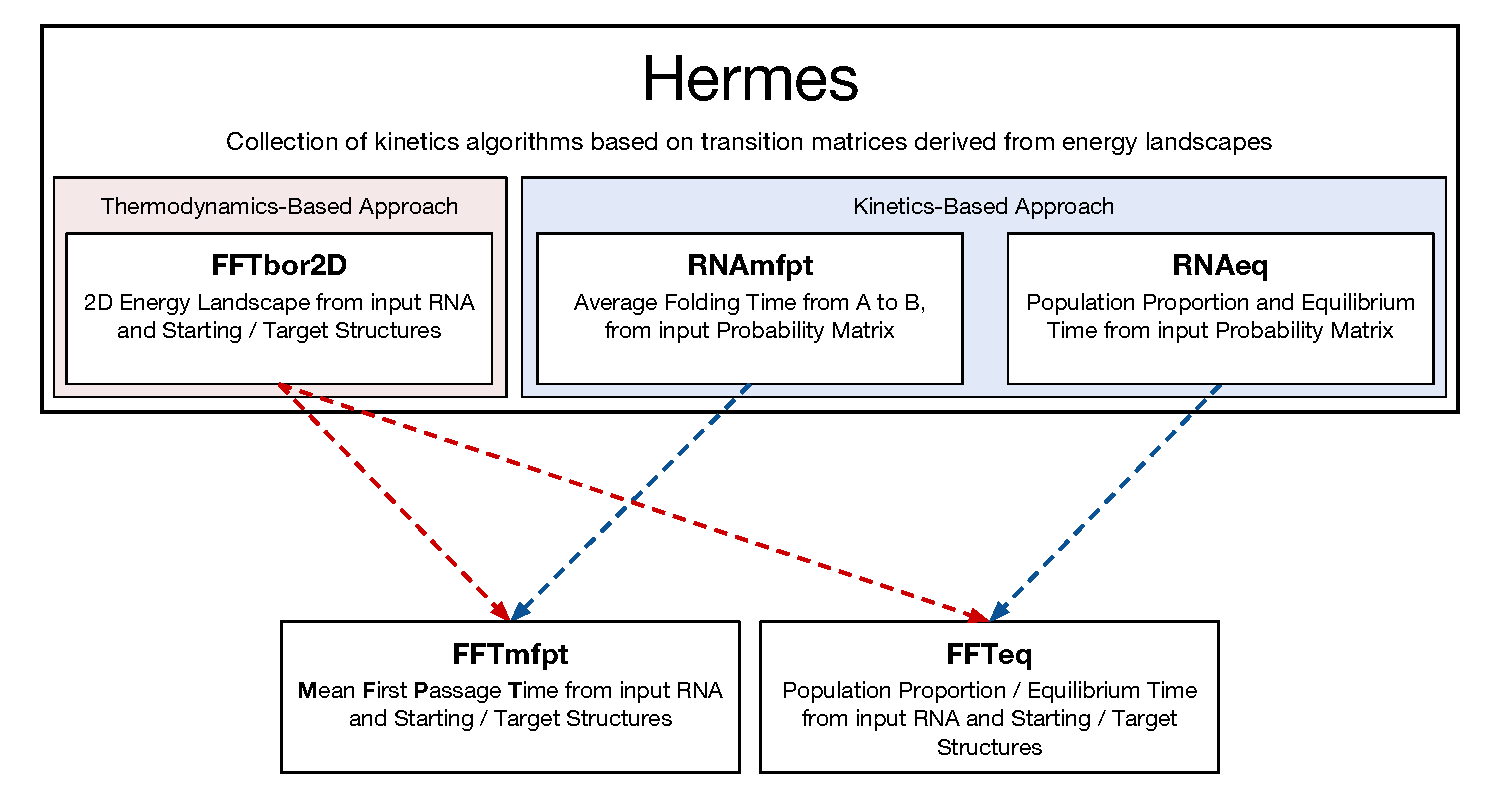
\includegraphics[width=.9\textwidth]{Figures/Hermes/softwareOrg.pdf}
\caption[Overall organization of the \hermes software suite]{Overall
organization of
\hermes. \ffttwo, \rnamfpt, and \rnaeq are three distinct software
packages we have developed, which compile into both standalone
executables and archive files, providing an API that allow novel
applications development using source from each of the packages,
without having to copy-and-paste relevant functions. The applications
\fftmfpt and \ffteq are C++ wrappers that use data structures and functions from
\ffttwo, \rnamfpt and \rnaeq. \fftmfpt computes the
\mfpt (MFPT) for an RNA secondary structure to fold from an
initial structure, such as the empty structure or a given metastable
structure, into a target structure, such as the \mfe
(MFE) structure or possibly the Rfam \citep{Gardner.nar11} consensus
structure. \ffteq uses spectral decomposition to compute the \eqt and the
fraction of the population of RNA structures that are
equal to a given target structure, as a function of time.
}
\label{fig:hermes:organizationHermes}
\end{figure}

\subsection{Exact \mfpt with \rnamfpt}
\label{subsec:hermes:rnamfpt}

\rnamfpt computes the \mfpt (MFPT), sometimes
referred to as the \hit of a Markov chain, by using
matrix inversion \citep{meyermfpt}---see
\Secref{subsec:hermes:mfpt}. The program takes as input a
comma separated value (CSV) file containing the non-zero positions and
values of a \twoD probability grid; i.e. a CSV format file having columns {\em i},
{\em j}, and {\em p}. The first two columns, {\em i} and {\em j}
correspond to the $0$-indexed row-ordered position in the probability grid, and
the final column {\em p} is the stationary probability $p_{i,j}$.
From this input, the probability transition matrix is constructed using
\eqnref{hermes:xitionProbFfttwoWithoutHastings} and the
\mfpt is computed by matrix inversion.

Given RNA sequence \seq and secondary structure $x$,
let $N(x)$ denote the set of neighboring secondary structures of
\seq, whose \bpd with $x$ is one. Define the Markov
chain $\mathcal{M}(\seq)=(\str,P)$, where \str denotes the
set of all secondary structures of \seq, $\pSt(x)$ is the stationary
probability of structure $x$, defined by $\pSt(x)=\boltzf{x}/\fullZ$,
$\fullZ=\sum_{x} \boltzf{x}$, and the transition probability matrix $P
= (p_{x,y})$ is defined either with or without the Hastings
modification as follows.

{\em With the Hastings modification},

\begin{align}
\label{eq:hermes:xitionProbWithHastings}
p_{x,y}=
\begin{cases}
\frac{1}{|N(x,y)|} \cdot \min\left(1, \frac{\pSt(y)}{\pSt(x)} \cdot
\frac{N(x)}{N(y)}\right) & \text{if $y \in N(x)$} \\
0 &\text{if $x \ne y, y \not\in N(x)$} \\
1 - \sum_{k \in N(x)} p_{x,k} & \text{if $x=y$} \\
\end{cases}
\end{align}

{\em Without the Hastings modification},

\begin{align}
\label{eq:hermes:xitionProbWithoutHastings}
p_{x,y}=
\begin{cases}
\frac{1}{|N(x,y)|} \cdot \min\left(1, \frac{\pSt(y)}{\pSt(x)}\right)
& \text{if $y \in N(x)$} \\
0 &\text{if $x \ne y, y \not\in N(x)$} \\
1 - \sum_{k \in N(x)} p_{x,k} & \text{if $x=y$} \\
\end{cases}
\end{align}

The exact value of \mfpt (MFPT) can be computed as
follows. Let $x_0$ [resp. $x_{\infty}$] denote the empty structure
[resp. MFE structure] for sequence \seq (here we have implicitly
identified integer indices with secondary structures). Let
$\widetilde{P}_{x_{\infty}}$ be the matrix obtained from $P$ by
removal of the row and column with index $x_{\infty}$, and $I$ denote
the $(n-1)\times(n-1)$ identity matrix, where $n=|\str|$ is the
number of secondary structures of \seq. Let $e$ denote the vector of
size $n-1$, each of whose coordinates is $1$. It is well-known
\citep{meyermfpt} that for each $k\ne x_{\infty}$, the $k$th coordinate
of the vector $(I - \widetilde{P}_{x_{\infty}})^{-1} \cdot {\bf e}$ is
exactly equal to the \mfpt from the structure with
index $k$ to the target structure $x_{\infty}$. In particular, the
MFPT from the empty structure to the MFE structure is computable by
applying matrix inversion using a computational library such as the GSL.

Since this computation of the
\mfpt is mathematically exact, we consider that MFPT
to be the {\em gold standard} value for RNA folding kinetics.

Because this program was designed with the original intent
of handling \twoD probability grids, all vertexes are uniquely identified
by index tuples (which conceptually correspond to positioning in a \twoD
array). However, it is trivial to use this code with both
1D-probability grids such as those produced by \fftbor
\citep{senter.po12} or arbitrary transition matrices without any change
to the underlying implementation. The software additionally provides
many options for defining the format of the input as well as the
structure of the graph underlying the
Markov chain.

Due to our interest in efficiently estimating MFPT using coarse-grained \twoD
energy landscapes, the default input for \rnamfpt (and \rnaeq) is a \twoD
probability grid, as described above. We additionally allow as alternative input
an energy landscape (whereby transition probabilities are defined as in
equation \ref{eq:hermes:mfptXitionProb}).
Some of the options to influence the underlying transition matrix
include the option to force a fully
connected graph (useful in cases where there is no non-zero path
between the start / end state) or to enforce detailed balance.
Finally, \rnamfpt also accepts as input the probability transition matrix,
a stochastic matrix with row sums equal to 1, and computes the mean
first passage time for the corresponding Markov chain.

\subsection{Approximate \mfpt with \fftmfpt}
\label{subsec:hermes:fftmfpt}

\fftmfpt approximates the \mfpt of a given RNA
sequence folding from input structure \strA to \strB, by
computing {\em exactly} the \mfpt from state $(0,d_0)$ to state
$(d_0,0)$ in the \twoD probability grid obtained from running
\ffttwo. Here, $d_0$ is the \bpd between structures
\strAB, and the MFPT is computed for the Markov chain, whose states are
the non-empty \twoD probability grid points, and whose transition
probabilities are defined by $p_{(x,y),(x',y')} =
\frac{P(x',y')}{P(x,y)}$.

More formally, given an RNA sequence \seq, starting structure \strA, and
target structure \strB, we proceed in the following fashion. Let \dBP{\strA}{\strB} denote the \bpd between structures
\strAB. Then $\bfZ{}{x,y} = \sum_\str \boltzf{\str}$, where the sum is over
structures \str, such that $\dBP{\strA}{\str} = x$, and
$\dBP{\strB}{\str} = y$; as
well the partition function $\fullZ = \sum_\str \boltzf{\str}$, where the sum
is over all secondary structures \str of the sequence \seq.

Let $d_0= \dBP{\strA}{\strB}$, the \bpd between initial structure
\strA and target structure \strB.  Let $n$ denote the length of sequence \seq.
Define the Markov chain $\mathcal{M}_1(\seq) = (Q_1,P_1)$, where

\begin{align}
\label{eq:hermes:markovChainDef}
\begin{split}
Q_1 =\;& \{ (x,y) : 0 \leq x,y \leq n, (x+y \bmod 2)
= (d_0 \bmod 2), \\
& (d_0 \leq x+y), (x \leq d_0 + y), (y \leq d_0 + x) \}.
\end{split}
\end{align}

For reference, we say that the {\em parity condition} holds for
$(x,y)$ if

\begin{align}
\label{eq:hermes:parityCondition} (x+y \bmod 2) = (d_0 \bmod 2).
\end{align}

We say that the {\em triangle inequality} holds for $(x,y)$ if

\begin{align}
\label{eq:hermes:triangleInequality} (d_0 \leq x+y), (x \leq d_0 + y), (y
\leq d_0 + x)
\end{align}

Since we allow transitions between secondary structures that differ by
exactly one base pair, Markov chain transitions are allowed to occur
only between states $(x,y),(u,v) \in Q_1$, such that $u=x\pm 1$, $v =
y \pm 1$. However, we have found that for some RNA sequences, there is
no non-zero probability path from $(0,d_0)$ to $(d_0,0)$
(corresponding to a folding pathway from structure \strA to
\strB). Since \ffttwo computes probabilities $p(x,y)$ by
polynomial interpolation using the \fft, any
probability less than $10^{-8}$ is set to $0$. Also with \rnatwofold,
it may arise that there is no non-zero probability path
from structure $(0,d_0)$ to $(d_0,0)$.

To address this situation, we proceed as follows. Let $\epsilon =
10^{-8}$ and for all $(x,y) \in Q_1$, modify probabilities $p(x,y)$ by

\begin{align}
\label{eq:hermes:mfptNormalize} p(x,y) = \frac{p(x,y) +
\epsilon/|Q_1|}{1+\epsilon }.
\end{align}

This operation corresponds to adding the negligeable value of
$\epsilon=10^{-8}$ to the total probability, thus ensuring that there
are paths of non-zero probability between any two states. After this
$\epsilon$-modification and renormalization, {\em when using the
Hastings modification}, the transition probabilities $P((u,v)|(x,y))$
are given by

\begin{align}
\label{eq:hermes:xitionProbFfttwoWithHastings}
P((u,v)|(x,y))=
\begin{cases}
\frac{1}{|N(x,y)|} \cdot \min\left(1, \frac{p(u,v)}{p(x,y)} \cdot
\frac{N(x,y)}{N(u,v)}\right) & \text{if $(u,v) \in N(x,y)$} \\
0 &\text{if $(u,v) \ne (x,y), (u,v) \not\in N(x,y)$} \\
1 - \sum_{(k,\ell) \in N(x,y)} P((k,\ell)|(x,y)) & \text{if $(u,v)=(x,y)$} \\
\end{cases}
\end{align}

Here the set $N(x,y)$ of adjacent neighbors is defined by $N(x,y) = \{
(u,v) \in Q_1 : u = x \pm 1, v = y \pm 1 \}$, and the stationary
probability $p(x,y)$ is obtained from \ffttwo.

{\em Without the Hastings modification}, the transition probabilities
$P((u,v)|(x,y))$ are instead given by

\begin{align}
\label{eq:hermes:xitionProbFfttwoWithoutHastings}
P((u,v)|(x,y))=
\begin{cases}
\frac{1}{|N(x,y)|} \cdot \min\left(1, \frac{p(u,v)}{p(x,y)}\right)
& \text{if $(u,v) \in N(x,y)$} \\
0 &\text{if $(u,v) \ne (x,y), (u,v) \not\in N(x,y)$} \\
1 - \sum_{(k,\ell) \in N(x,y)} P((k,\ell)|(x,y)) & \text{if $(u,v)=(x,y)$} \\
\end{cases}
\end{align}

As we report in \Secref{subsec:hermes:corr},
given an RNA
sequence \seq, if \strA is the empty structure and \strB the MFE
structure of \seq, then \fftmfpt output is well correlated with the
exact MFPT in folding the empty structure to the MFE structure, where
transitions between structures involve the addition or removal of a
single base pair.

\subsection{Exact \eqt with \rnaeq}
\label{subsec:hermes:rnaeq}

\rnaeq computes the population proportion of a user-provided structure
over arbitrary time units. Like \rnamfpt, this program takes as input a
comma separated value (CSV) file containing the non-zero positions and
values of a \twoD probability grid. From this input a rate matrix
is constructed for the underlying Markov process. Alternatively,
\rnaeq can accept as input an arbitrary rate matrix. Performing
spectral decomposition of the column-ordered rate matrix that
underlies the corresponding Markov process, \rnaeq computes either
the \eqt or population occupancy frequencies.

Define the continuous Markov process
$\mathcal{M}=(\str,R)$, where \str is defined as in
\Secref{subsec:hermes:rnamfpt}, $R$ is the {\em rate matrix} defined by

\begin{align}
\label{eq:hermes:xitionRateWithoutHastings}
k_{x,y}=
\begin{cases}
\min\left(1, \frac{\pSt(y)}{\pSt(x)}\right)
& \text{if $y \in N(x)$} \\
0 &\text{if $x \ne y, y \not\in N(x)$} \\
- \sum_{k \in N(x)} p_{x,k} & \text{if $x=y$} \\
\end{cases}
\end{align}

Clearly the rate matrix satisfies detailed balance; i.e. $\pSt(x)
\cdot k_{x,y} = \pSt(y) \cdot k_{y,x}$ for all distinct $x,y \in
\str$. In fact, the rate matrix for Markov processes is usually
defined as above, precisely to ensure detailed balance, which then
implies that all eigenvalues of the rate matrix are real, thus
permitting explicit solution of the population occupancy frequency for
all states. We additionally considered a Hastings correction
for the rate matrix, where $k_{x,y} = \min(1, \frac{\pSt(y)}{\pSt(x)}
\cdot \frac{N(x)}{N(y)})$. The correlation in
Table \ref{table:correlationHermes} for equilibrium time computed from this
modified rate matrix is somewhat better than without the Hastings
correction. However, the Hastings correction is never used for rate
matrices, hence we only consider the usual definition of rate matrix
given in \eqnref{hermes:xitionRateWithoutHastings}.

\rnaeq can additionall call the
Vienna RNA Package program \rnasub \citep{wuchty.b99}, with a
user-specified upper bound to the energy difference with the minimum
free energy. With this option, the rate matrix is
constructed for the Markov process, whose states consist of all
the structures returned by \rnasub, and the \eqt or
population occupancy frequencies are computed. Due to the time
and memory required for this option, we do not expect it to be used except for
small sequences.

\subsection{Approximate \eqt with \ffteq}
\label{subsec:hermes:ffteq}

\ffteq allows an investigator to efficiently estimate population
kinetics for a sequence folding between two arbitrary, but fixed,
structures. The transition rate matrix underlying the Markov process
necessary for eigendecomposition is derived from the \twoD energy
landscape.
Indices $(x,y)$ in the rate matrix correspond to all strucutres having
\bpd $x$ [resp. $y$] to input structure \strA [resp. \strBresp],
which makes the graph size more tractable than structural
sampling with \rnasub using \rnaeq, even with constraints.

This method consists of computing the equilibrium time
from the master equation for the coarse-grain Markov process
$\mathcal{M}=(Q_1,R)$, where $Q_1$ is defined in
\eqnref{hermes:markovChainDef}, and the rate matrix
$R = (k((x,y),(u,v)))$ is defined by

\begin{align}
\label{eq:hermes:xitionRateFfttwoWithoutHastings}
k((u,v),(x,y))=
\begin{cases}
\min\left(1, \frac{p(u,v)}{p(x,y)}\right) & \text{if $(u,v) \in N(x,y)$} \\
0 &\text{if $(u,v) \ne (x,y), (u,v) \not\in N(x,y)$} \\
- \sum_{(k,\ell) \in N(x,y)} P((k,\ell)|(x,y)) & \text{if $(u,v)=(x,y)$} \\
\end{cases}
\end{align}

Equilibrium time is then computed for this Markov process using
\eqnref{hermes:populationOccupancyEquation}.

\subsubsection{Population occupancy curves with \ffteq}
\label{subsubsec:hermes:popcurve}

Population occupancy curves provide valuable visual insight into the folding
kinetics of RNA molecules.
A computation for the probability distribution
$p(t) = (p_1(t),\dots,p_n(t))^{\text T}$ of all states $1 \leq x \leq n$ at
time $t$ is described in \eqnref{hermes:solutionMasterEquationForSingleState}.
Rather than plot $p(t)$ as a function of $t$, we find it more
visually impactful to plot the log-logistic function $p(\log_{10}(t))$,
yielding the curvess seen in \Figref{hermes:populationOccupancySplicedLeader}.

\begin{figure}[!ht]
\centering
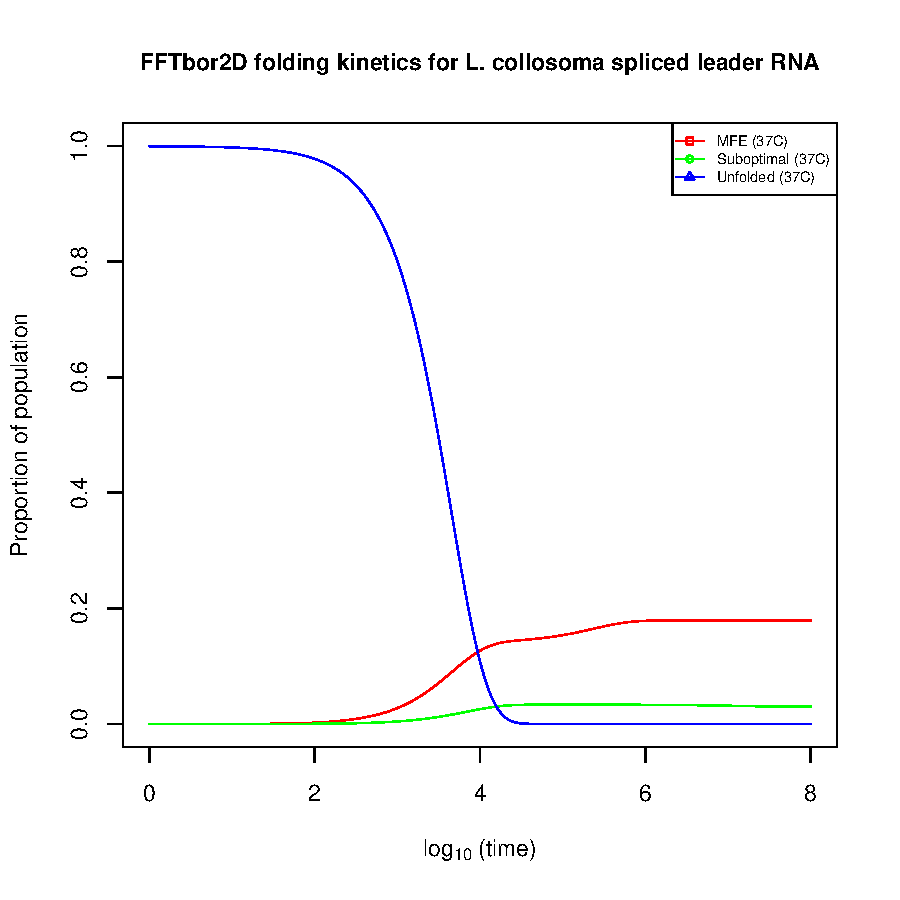
\includegraphics[width=0.7\textwidth]{Figures/Hermes/populationOccupancyCurves.pdf}
\caption[Population occupancy curves computed with \ffteq for the
$56$ nt conformational switch {\em L. collosoma} spliced leader RNA]{
Population occupancy curves computed with \ffteq for the
$56$ nt conformational switch {\em L. collosoma} spliced leader RNA,
with sequence \ms{AACUAAAACAAUUUUUGAAGAACAGUUUCUGUACUUCAUUGGUAUGUAGA}
GACUUC. The dot bracket format for the MFE structure, as computed by
version $2.1.7$ of \ms{RNAfold -d0}, is
\strfont{.......................((((((((((((.....)))))..)))))))..} with free
energy \kmol{-8.6}, while that of the the alternate suboptimal
structure is
\strfont{..((...((((((..(((((.((((...)))).)))))..))).)))..)).....} with free
energy \kmol{-7.5}. In the case of the MFE structure, the
equilibrium occupancy $P(t_{\infty})$, which \hermes approximates
as $0.1789$ should equal the Boltzmann probability $0.1791$,
since the MFE structure is the only structure at distance $x_0$ [resp.
$y_0$] from the reference structures \strA (empty
structure) [resp. \strB (MFE structure)]. As well, if there are few
other low energy structures at the same \bpd $x_1$
[resp. $y_1$] from \strA [resp. \strBresp] as that of the alternate suboptimal
structure, then we expect that the occupancy probability $0.0300$
for the $(x_1,y_1)$ be approximately the Boltzmann probability
$0.0301$ of the alternate structure.}
\label{fig:hermes:populationOccupancySplicedLeader}
\end{figure}

\subsubsection{Approximating \eqt from occupancy curves}
\label{subsubsec:hermes:eqestimate}

The computation of an \eqt value from the eigendecomposition of the rate matrix
is a rather thorny issue. While in principle a nonlinear solver can be used to
compute the \eqt $t$ (from equation \ref{eq:hermes:solutionEquilibriumTime}),
in practice due to what we believe to be numeric instability issues the approach
was intractable. For this reason, we estimate the \eqt from the population
occupancy curve, an approach also taken by \treekin
\citep{wolfingerstadler:kinetics}. Our first
approximation of \eqt involved using a sliding window approach, where we
compute the smallest $t_0$,
such that for $t \in \{t_0+\tD,t_0+2\tD,t_0+3\tD,\dots,t_0+(w-1)\cdot\tD\}$, the absolute difference
$|p(t)[\xEnd] - p(t_0)[\xEnd]| < \epsilon$, for $\epsilon =
10^{-4}$ and step size \tD across a window of length $w$. In systems where there are local energy minima, this approach has the
drawback of prematurely indicating equilibrium, as seen in
\Figref{hermes:eqEstFromRnaEq}. To address this concern, we introduce the
concept of $\delta,\epsilon$ equilibrium.

Given a starting state $i'$, target state $i$, and user definable parameters
$w = 5, \tD = 10^{-3}, \delta = 10^{-3}$ and $\epsilon = 10^{-4}$, we compute the estimated
equilirium using the following algorithm.
\medskip

\begin{figure}[!ht]
\hrule \rule[0ex]{0pt}{0pt}
\begin{center}
{\large Pseudocode for estimating equilibrium time} \\
\end{center}
\begin{tabular*}{\textwidth}{ll}
{\sc Purpose:} & Estimate time $\log_{10}(t)$ at which state \xStart appears
within $\epsilon$ of equilibrium \rule[-1.5ex]{0pt}{0pt} \\
{\sc Input:} & States \xStart, \xEnd; \tMin, \tMax;
$w = 5, \tD = 10^{-3}, \delta = 10^{-3}, \epsilon = 10^{-4}$ \rule[-1.5ex]{0pt}{0pt} \\
{\sc Output:} & Time $\log_{10}(t)$ at which $p_{\xEnd}(10^t)$ varies by no
more than $\epsilon$ within a \\ & window of size $w$, having step size \tD
\rule[-1.75em]{0pt}{0pt} \\
\hline \rule[0ex]{0pt}{0pt}
\end{tabular*}
\begin{algorithmic}[1]
\Function{EstimateEquilibrium}{\xStart, \xEnd, \tMin, \tMax, \tD, $\delta$, $\epsilon$, $w$}
\State $t \gets \Call{SoftBound}{\xEnd, \tMin, \tMax, \tD, \delta, s}$
\If{$\Call{WindowEq}{\xEnd, t, \tD, w, \epsilon}$}
\While{$t > \tMin$ AND $\Call{WindowEq}{\xEnd, t, \tD, w, \epsilon}$}
\State $t \gets t - \tD$
\EndWhile
\EndIf
\While{$t < \tMax$ AND NOT $\Call{WindowEq}{\xEnd, t, \tD, w, \epsilon}$}
\State $t \gets t + \tD$
\EndWhile
\If{$t = \tMin$}
\Comment{$x$ doesn't leave equilibrium after \tMin}
\State \textbf{return} $-\infty$
\ElsIf{$t = \tMax$}
\Comment{$x$ doesn't reach equilibrium before \tMax}
\State \textbf{return} $\infty$
\Else
\State \textbf{return} $t$
\EndIf
\EndFunction
\algstore{eqEst}
\end{algorithmic}
\rule[0ex]{0pt}{1.5em} \hrule
\end{figure}
\clearpage

\begin{figure}[!ht]
\begin{algorithmic}[1]
\algrestore{eqEst}
\Function{SoftBound}{$i$, \tMin, \tMax, \tD, $\delta$, $s$}
\State $i_{\infty} \gets p_i(10^{\tMax})$
\Comment{From \eqnref{hermes:solutionMasterEquationForSingleStateFixedStartPop}}
\State $t \gets \tMin + \frac{\tMax - \tMin}{2}$
\State $t' \gets \tMax$
\While{$|t - t'| > \tD$}
\Comment{Binary search for time $t$ within $\delta$ of \tMax}
\State $t_{\text{temp}} \gets t$
\If{$|p_i(10^t) - p_i(10^{t'})| > \delta$}
\State $t \gets t + s * \frac{|t - t'|}{2}$
\Comment{$s$ is $1$ [resp. $-1$] for the right [resp. left] bound}
\Else
\State $t \gets t - s * \frac{|t - t'|}{2}$
\EndIf
\State $t' \gets t_{\text{temp}}$
\EndWhile
\State \textbf{return} $t$
\EndFunction
\Function{WindowEq}{$x$, $t$, \tD, $w$, $\epsilon$}
\Comment{Is $x$ within $\epsilon$ over $[t, t+(w-1)\cdot\tD]$}
\For{$i \gets 1, w - 1$}
\If{$|p_x(10^{t+i\cdot\tD}) - p_x(10^t)| > \epsilon$}
\State \textbf{return} \textbf{false}
\EndIf
\EndFor
\State \textbf{return} \textbf{true}
\EndFunction
\rule[-0.35ex]{0pt}{0pt}
\end{algorithmic}
\caption[Pseudocode for estimating equilibrium time]{The function {\sc EstimateEquilibrium} computes the smallest $t_0 > t'$,
such that for $t \in \{t_0+\tD,t_0+2\tD,t_0+3\tD,\dots,t_0+(w-1)\cdot\tD\}$,
the absolute difference $|p(t)[\xEnd] - p(t_0)[\xEnd]| < \epsilon$ and
$|p(t')[\xEnd] - p(\tMax)[\xEnd]| \approx \delta|$. If $t'$ is already in
equilibrium, we relax the constraint that $t_0 > t'$ and instead find the
first $t_0 < t'$ that satisfies the equilibrium requirements within the window
$w$. {\sc SoftBound} is a helper function that uses binary search to find the
starting time $t'$ from which the window starts. {\sc WindowEq} returns a
boolean value if the state of interest $x$ varies by no more than $\epsilon$
across the window $w$ starting at time $t$.}
\label{fig:hermes:eqEst}
\rule[0ex]{0pt}{1.5em} \hrule
\end{figure}

In using the approach outlined in \Figref{hermes:eqEst}, the root-mean-square
deviation (RMSD)
between $p_{\xEnd}(t_0)$ and $\frac{\boltzf{\xEnd}}{\fullZ}$ is $0.0041$, where
RMSD is defined as

\begin{align}
\label{eq:hermes:rmsd}
\sqrt{\frac{\sum_{i=1}^{n} (\widehat{x_i} - x_i)^2}{n}}.
\end{align}

Visual inspection of the estimated equilibrium times
(\Figref{hermes:eqEstFromRnaEq}) are much better than the
na\"{\i}ve approach used by \treekin, which uses a simple sliding window for
all $x \in Q$.
We also allow defining the \eqt to be the
smallest $t_0$, such that for
$t \in \{t_0+\tD,t_0+2\tD,t_0+3\tD,\dots,t_0+(w-1)\cdot\tD\}$, the
absolute difference $|p(t)[x] - p(t_0)[x]| < \epsilon$ for all $x \in
Q$ using Algorithm \ref{fig:hermes:eqEst};
however, results suggest that this definition is inferior
to the consideration of a single single target state $i$,
perhaps due to numerical instability issues when
$Q$ is taken to be the set of all secondary structures for sequences in
the benchmarking set described later.

\begin{figure}[!ht]
\centering
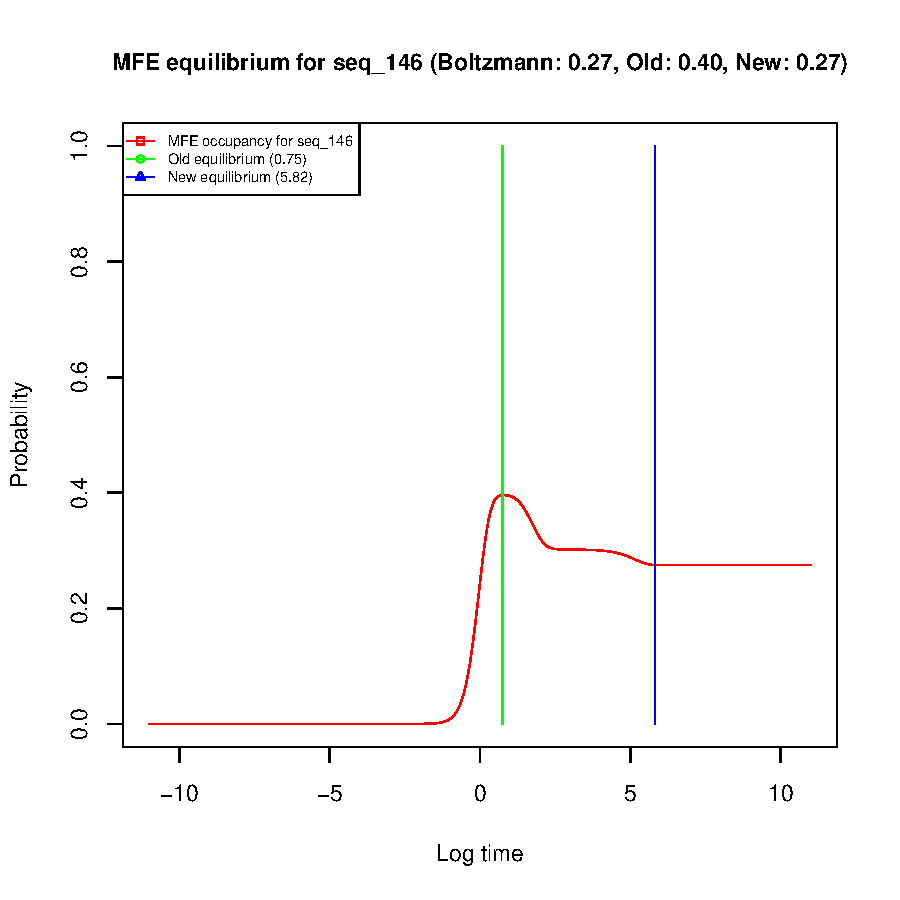
\includegraphics[width=0.45\textwidth]{Figures/Hermes/eqEstFromRnaEqSeq146.pdf}
\quad
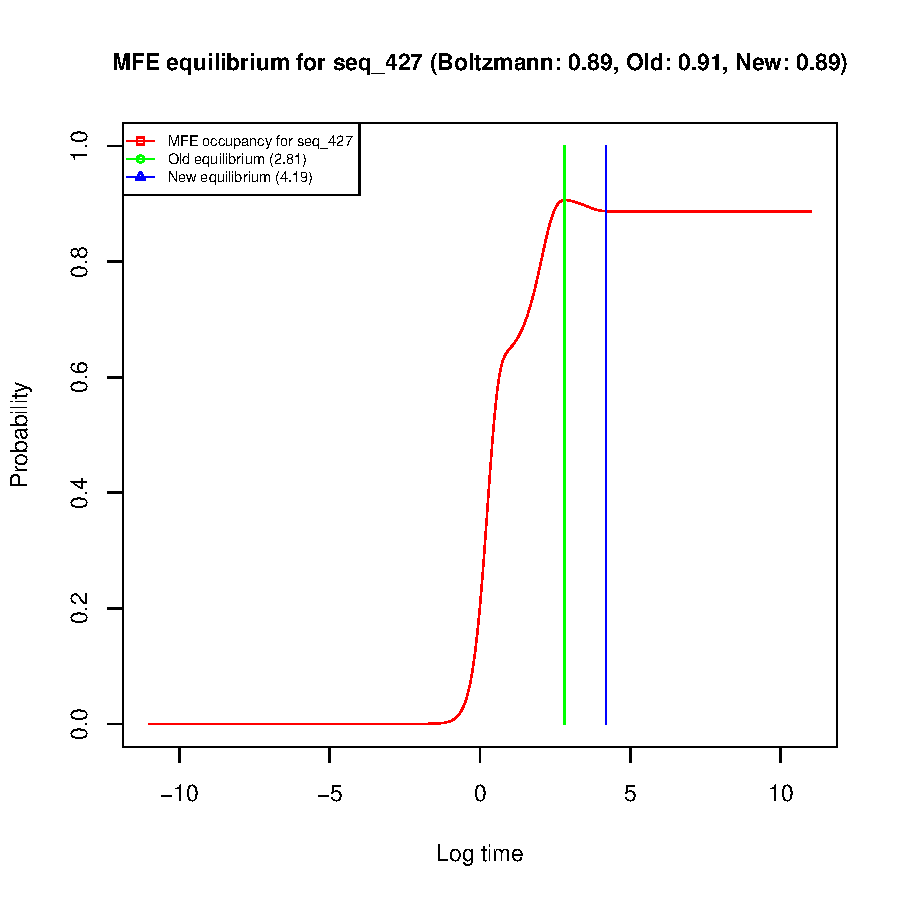
\includegraphics[width=0.45\textwidth]{Figures/Hermes/eqEstFromRnaEqSeq427.pdf}
\caption[Example of the differences in using a sliding window approach for estimating \eqt versus a more robust approach, outlined in Algorithm \ref{fig:hermes:eqEst}]{Example of the differences in using the simple sliding window
approach (green) versus the approach outlined in Algorithm \ref{fig:hermes:eqEst}
(blue). There are two representative sequences shown from the benchmarking
dataset described in \Secref{sec:hermes:benchdata}, sequence \#$146$
{\em (Left)} and \#$427$ {\em (Right)}. Note that the $p(t)$ for the approach from
Algorithm \ref{fig:hermes:eqEst} is much closer to the computed Boltzmann
probability---the root-mean-square deviation (RMSD, equation
\ref{eq:hermes:rmsd}) across the dataset of $1,000$ sequences is $0.0041$
[resp. $0.0491$] for the approach described in Algorithm \ref{fig:hermes:eqEst}
[resp. simple sliding window].}
\label{fig:hermes:eqEstFromRnaEq}
\end{figure}

\section{Benchmarking data for computational comparison}
\label{sec:hermes:benchdata}

In this section, we describe a
benchmarking set of $1,000$ small RNAs used to benchmark the previously
described kinetics methods in a comparative study. To ensure that mean
first passage time can be computed from
$(I - P^{-}_{\xEnd})^{-1} \cdot {\bf e}$ by using matrix
inversion, that spectral decomposition of the rate matrix is possible,
and to ensure that \kinfold simulations would provide sufficient
statistics, we generated a collection of $1,000$ random RNA sequences of
length $20$ nt, each having expected compositional frequency of $1/4$
for A,C,G,U, and each having at most $2,500$ distinct secondary
structures, such that the \mfe is less than or equal to
\kmol{-5.5}.

For example, one of the $1,000$ sequences is \ms{ACGCGACGUGCACCGCACGU} with
\mfes \strfont{.....((((((...))))))} having free
energy of \kmol{-6.4}. Statistics for the free energies of the
$2,453$ secondary structures of this $20$-mer are the following: mean is
$10.695$, standary deviation is $4.804$, maximum is $25.00$, minimum
is $-6.40$. A histogram for the free energy of all secondary
structures of \ms{ACGCGACGUGCACCGCACGU} is depicted in
the left panel of \Figref{hermes:plmv}. The right panel of the
same figure depicts the \mfes of the
$54$ nt hammerhead type III ribozyme from Peach Latent Mosaic Viroid
(PLMVd), discussed later. This secondary structure is identical
to the consensus structure from Rfam $11.0$ \citep{Gardner.nar11}.

\begin{figure}[!ht]
\centering
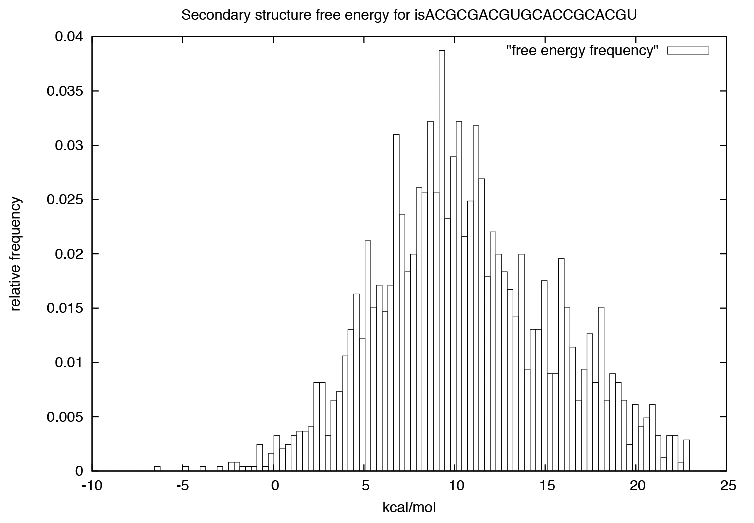
\includegraphics[width=0.525\textwidth]{Figures/Hermes/plmvDist.pdf}
\quad
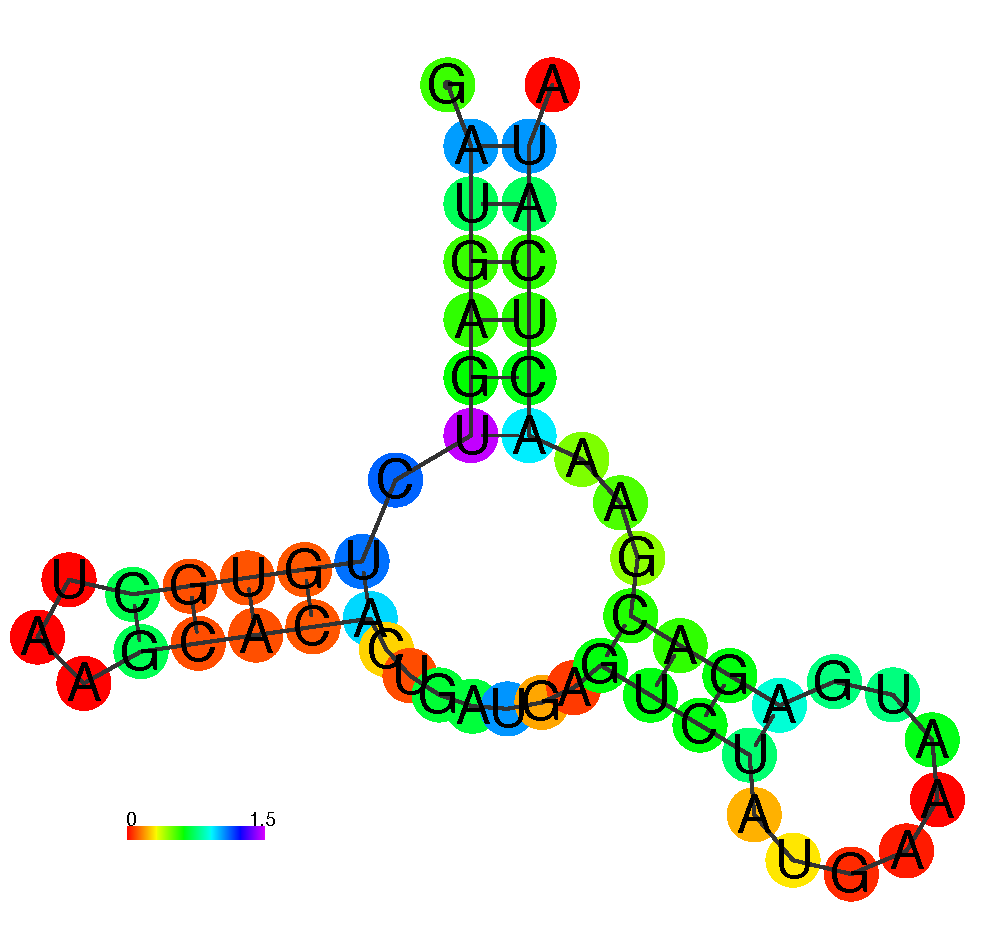
\includegraphics[width=0.375\textwidth]{Figures/Hermes/plmvStr.pdf}
\caption[{\em (Left)} Histogram of free energies of secondary structures of
an example $20$-mer from the benchmarking dataset.
{\em (Right)} Minimum free energy structure of the $54$ nt Peach Latent Mosaic
Viroid (PLMVd) AJ$005312.1$ $282$--$335$]{
{\em (Left)} Histogram of free energies of secondary structures of
\ms{ACGCGACGUGCACCGCACGU}, which range from $-6.5$ to \kmol{+25}, with
mean of \kmol{10.7}.
{\em (Right)} Minimum free energy structure of the $54$ nt Peach Latent Mosaic
Viroid (PLMVd) AJ$005312.1$ $282$--$335$, which is identical to the consensus
structure from Rfam $11.0$ \citep{Gardner.nar11}. \rfold from
Vienna RNA Package $2.1.7$ with energy parameters from the Turner $1999$
model were used, since the \mfes determined by
the more recent Turner $2004$ energy parameters
does {\em not} agree with the Rfam consensus structure---see
\citep{synthetichammerheads}. Positional entropy, a measure
of divergence in the base pairing status at each positions for the
low energy ensemble of structures, is indicated by color, using the
RNA Vienna Package utility script \ms{relplot.pl}.
}
\label{fig:hermes:plmv}
\end{figure}

\Figref{hermes:kinfoldMeanStdev} displays the mean
and standard deviation for \kinfold simulations of folding time
for each of the $1,000$ RNA sequences from our benchmarking data. For
each sequence, the mean and standard deviation of the time required to
fold the empty structure to the MFE structure were computed from
$10,000$ \kinfold runs, each run with an upper bound of $10^8$
Monte Carlo steps, thus ensuring that all simulations converged. The
sequences were then sorted by increasing folding time mean. Standard
deviation exceeded the mean in $83.9\%$ of the $1,000$ cases, indicating
the enormous variation between separate \kinfold runs, even for
$20$ nt RNA sequences having at most $2,500$ secondary structures.
Elementary considerations from statistics indicate that for our benchmarking set
of $20$-mers, the minimum sample size $n = \left( \frac{z_{\alpha/2}
\cdot \sigma}{E} \right)^2$ ranges from $937,712$ to $23,289,310$
to have a confidence level of $95$\% that the average of $n$
\kinfold runs differs from the real folding time by at most $100$ steps.
In our opinion, \kinfold is an expertly crafted implementation of
Gillespie's algorithm for an event driven Monte Carlo simulation of
one-step RNA secondary structure folding. From the standpoint of
biophysics and physical chemistry, there is no more reliable
simulation method, except of course the exact computation of mean
first passage time using linear algebra. Nevertheless, the enormous
time required for reliable \kinfold estimations and the large
standard deviations observed point out the need for a faster method to
approximate folding time.

With this in mind, it is natural to turn to coarse-grained models,
as done by Wolfinger et al. \citep{wolfingerstadler:kinetics} and by
Tang et al. \citep{tang.jmb08}. The software of Tang et al. appears not
to be available. Concerning the method of Wolfinger et al. (called
\barrierseq in our benchmarking), there is now a web server available,
which runs \rnasub \citep{wuchty.b99} to generate all secondary structures within
a user-specified energy range, then runs \barriers \citep{flammhofacker}
to generate basins of attraction around a user-specified number of locally
optimal structures, and then runs \treekin on the output of \barriers.
The program \treekin performs some of the same operations as \hermes,
by computing population occupation frequencies by spectral decomposition.
Nevertheless it would require a user to write scripts and perform
several manual steps, in order to determine the equilibrium time for
an input RNA sequence, with respect to the macrostate Markov process
of \citep{wolfingerstadler:kinetics}. In addition, because \barriers computes
basins of attraction by utilizing the output of \rnasub, estimating kinetics
for the refolding of an RNA molecule from the empty structure requires
exhaustive enumeration of all suboptimal structures having non-positive
free energy.

\begin{figure}[!ht]
\centering
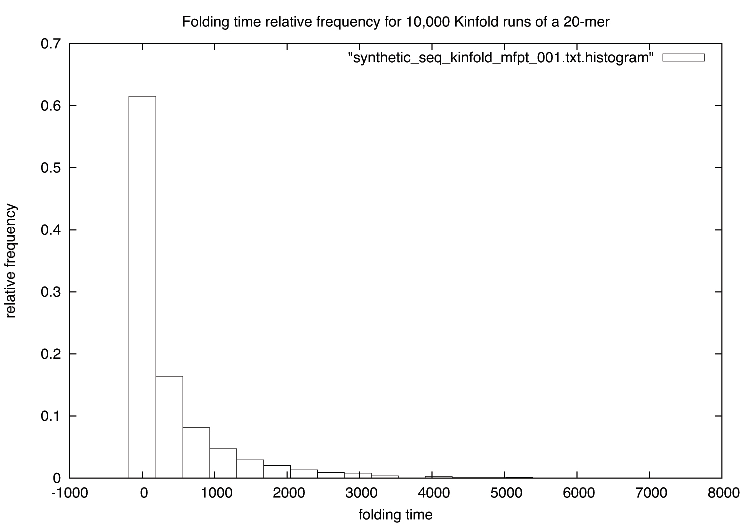
\includegraphics[width=0.45\textwidth]{Figures/Hermes/kinfoldTimeDist.pdf}
\quad
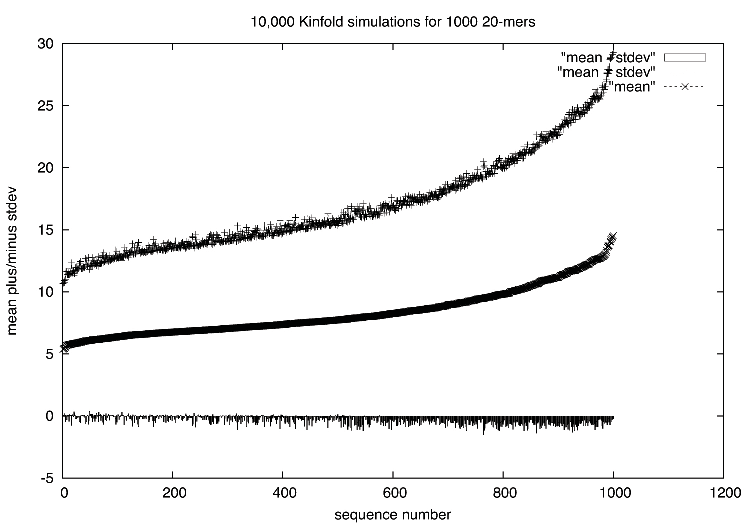
\includegraphics[width=0.45\textwidth]{Figures/Hermes/kinfoldMeanStdev.pdf}
\caption[Analysis of \kinfold folding times for $20$-mer
\ms{CCGAUUGGCGAAAGGCCACC}]{{\em (Left)} Histogram of \kinfold folding times for $20$-mer
\ms{CCGAUUGGCGAAAGGCCACC}. The mean [resp. standard deviation] of $10,000$ runs of \kinfold for this $20$-mer is $538.37$ [resp. $755.65$]. Note the close fit to the exponential distribution, {\em (Right)} Mean minus standard deviation ($\mu -\sigma$), mean ($\mu$), and mean plus standard deviation ($\mu + \sigma$) of the logarithm of \kinfold folding times, taken over $10,000$ runs for each of the $1,000$ sequences from the benchmarking set of $20$-mers. For graphical illustration, we have sorted the log folding times in increasing order.}
\label{fig:hermes:kinfoldMeanStdev}
\end{figure}

\subsection{Pearson correlation coefficients for various kinetics packages}
\label{subsec:hermes:corr}

In this section, we display the correlation between
\begin{inparaenum}[\em 1\upshape)]
\item the {\em gold standard} method \rnamfpt, both with and without the Hastings
modification using equations (\ref{eq:hermes:xitionProbWithHastings}) and
(\ref{eq:hermes:xitionProbWithoutHastings});
\item the {\em platinum standard} method \rnaeq, using
\eqnref{hermes:xitionRateWithoutHastings};
\item the {\em silver standard} method \kinfold;
\item \fftmfpt with and without the Hastings modification using equations
(\ref{eq:hermes:xitionProbFfttwoWithHastings}) and
(\ref{eq:hermes:xitionProbFfttwoWithoutHastings});
\item \ffteq which computes \eqt for the \twoD grid using
\eqnref{hermes:xitionRateWithoutHastings}; and finally
\item \rnatwofold with and without the Hastings modification using equations
(\ref{eq:hermes:xitionProbFfttwoWithHastings}) and
(\ref{eq:hermes:xitionProbFfttwoWithoutHastings}).
\end{inparaenum}
Correlations
with [resp. without] the Hastings modification are summarized in the
lower [resp. upper] triangular portion of
Table \ref{table:correlationHermes}. It is clear that correlations between
the mathematically exact methods \rnamfpt, \rnaeq, and
approximation methods \kinfold, \fftmfpt, \ffteq, \rnatwofold are
improved when using the Hastings correction.

Figures \ref{fig:hermes:scatterplotRnaEqVsRnaMfptHastingsAndKinfold},
\ref{fig:hermes:scatterplotRnaMfptHastingsVsKinfoldAndFftMfpt},
\ref{fig:hermes:scatterplotFftMfptVsKinfoldAndFftEq}
depict scatterplots for kinetics obtained by some of the algorithms
above. The left panel of
\Figref{hermes:scatterplotRnaEqVsRnaMfptHastingsAndKinfold}
shows a scatter plots for gold standard \rnamfpt versus platinum
standard \rnaeq, with correlation value $0.5652$. The right
panel of the same figure shows a scatter plot for \kinfold versus
\rnaeq, with correlation $0.7814$. Note the persence of two
clusters in this and some of the other scatter plots. Cluster A
consists of RNA sequences whose folding time, as determined by \rnamfpt
or \rnaeq, is rapid---specifically, the natural
logarithm of the MFPT is at most $7.5$. Cluster B consists of the
remaining RNA sequences, whose folding time is longer than that of
cluster A. There are no significant differences between RNA sequences
in clusters A and B with respect to GC-content, sequence logo, minimum
free energy, number of secondary structures, etc.  The left panel of
\Figref{hermes:scatterplotRnaMfptHastingsVsKinfoldAndFftMfpt}
shows the scatter plot for \rnamfpt versus \kinfold, with
correlation $0.7933$, and the right panel shows the scatter plot for
\rnamfpt versus \fftmfpt, with correlation $0.6035$.
\Figref{hermes:scatterplotFftMfptVsKinfoldAndFftEq}
shows scatter plots for \fftmfpt versus \kinfold {\em (Left)} and
for \fftmfpt versus \ffteq {\em (Right)}, with respective
correlation values $0.7608$ and $0.9589$. \kinfold obviously provides
a better correlation with the exact value of \mfpt;
however, since the standard deviation of \kinfold runs is as
large as the mean, accurate kinetics estimates
from \kinfold require prohibitively large computational time---indeed, in
\citep{wolfingerstadler:kinetics} reliable kinetics for phe-tRNA from
yeast were obtained by $9,000$ \kinfold simulations, each for $10^8$
steps, requiring $3$ months of CPU time on an Intel Pentium $4$ running at
$2.4$ GHz under Linux. Although the correlation value of $0.6035$ between
\rnamfpt and \fftmfpt is much less than that obtained by \kinfold,
the runtime required by our method \fftmfpt is measured
in seconds, even for moderate to large RNAs. For this reason, we
advocate the use of \fftmfpt in synthetic biology screens to
design RNA sequences having certain desired kinetic properties. Once
promising candidates are found, it is possible to devote additional
computational time to \kinfold simulations for more accurate
kinetics.

\begin{figure}[!ht]
\centering
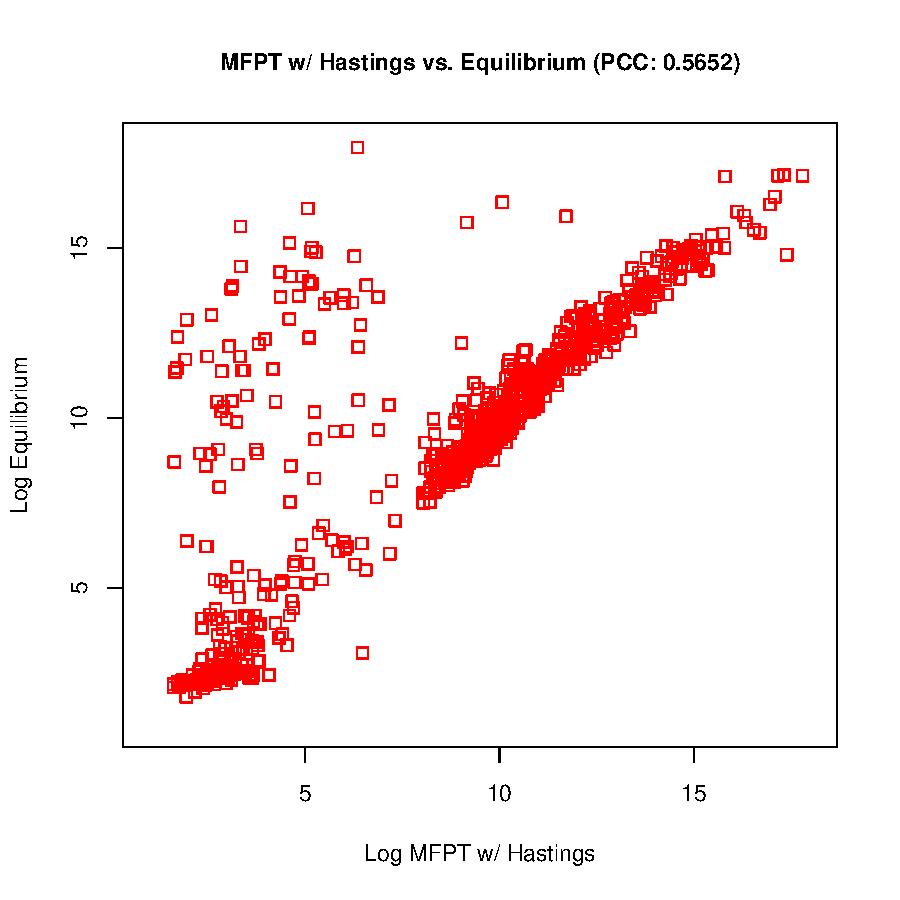
\includegraphics[width=0.45\textwidth]{Figures/Hermes/rnaMfptHastingsRnaEq.pdf}
\quad
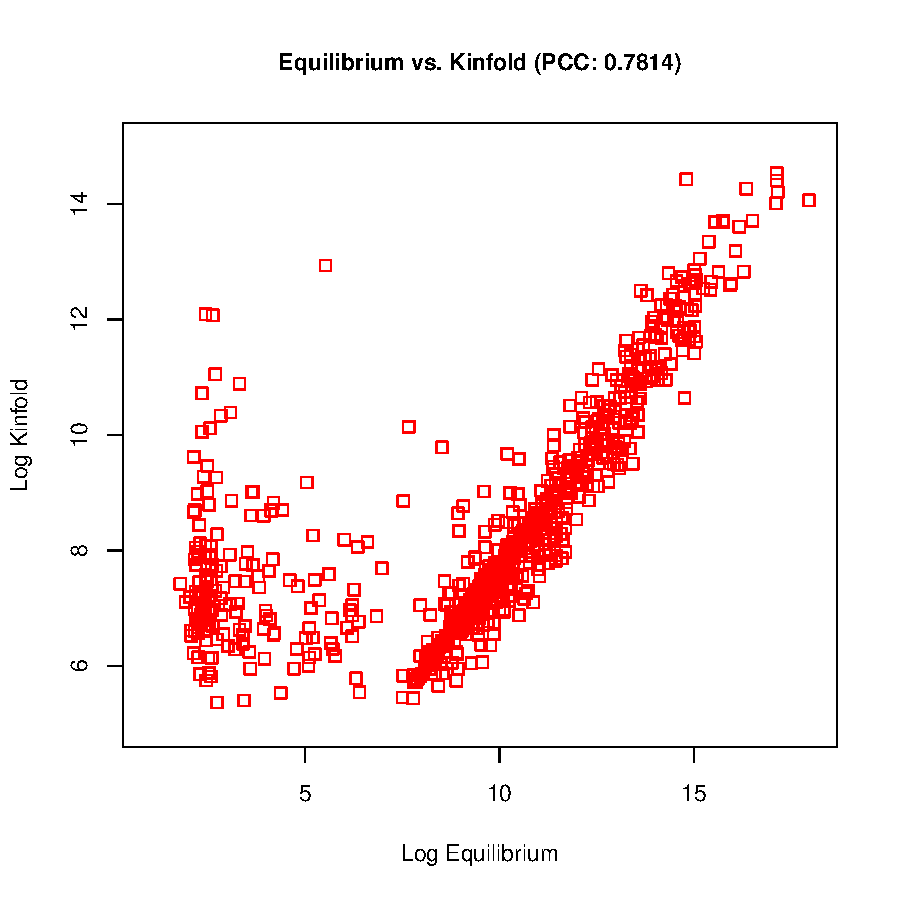
\includegraphics[width=0.45\textwidth]{Figures/Hermes/rnaEqKinfold.pdf}
\caption[Scatter plots of the natural logarithm of times from \rnamfpt
versus \msresp{RNAeq} {\em (Left)} and for \kinfold versus
\msresp{RNAeq} {\em (Right)}]
{Scatter plots of the natural logarithm of times from \rnamfpt
versus \msresp{RNAeq} {\em (Left)} and for \kinfold versus
\msresp{RNAeq} {\em (Right)}.}
\label{fig:hermes:scatterplotRnaEqVsRnaMfptHastingsAndKinfold}
\end{figure}

\begin{figure}[!ht]
\centering
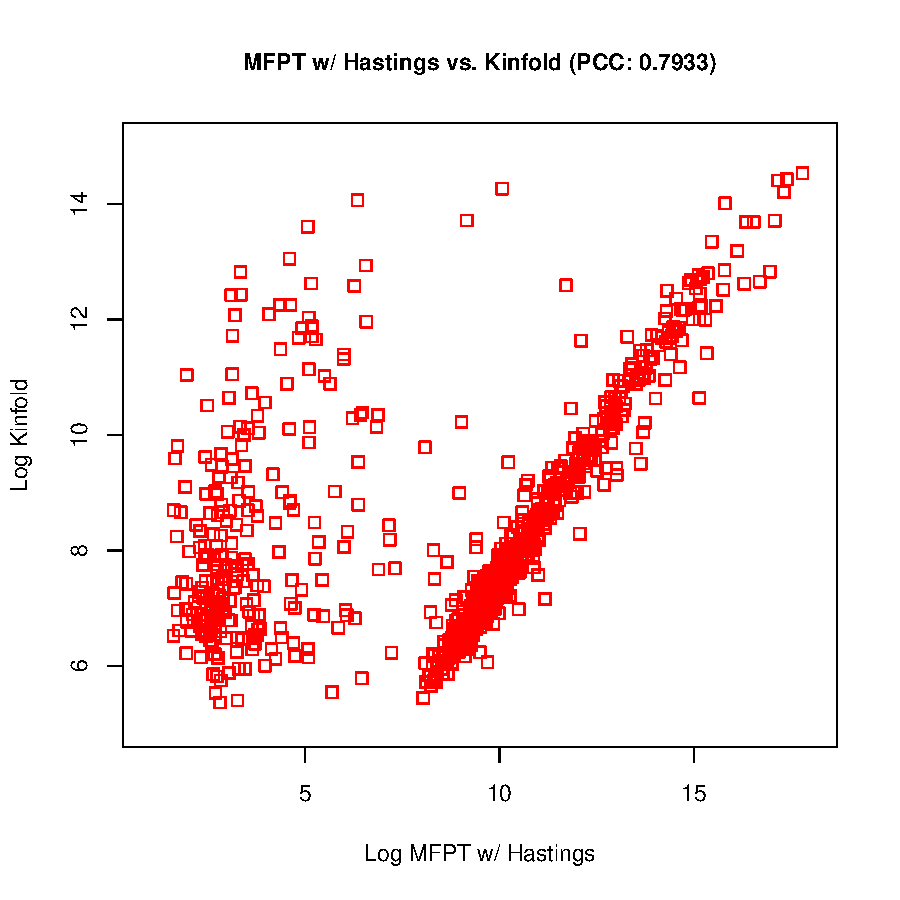
\includegraphics[width=0.45\textwidth]{Figures/Hermes/rnaMfptHastingsKinfold.pdf}
\quad
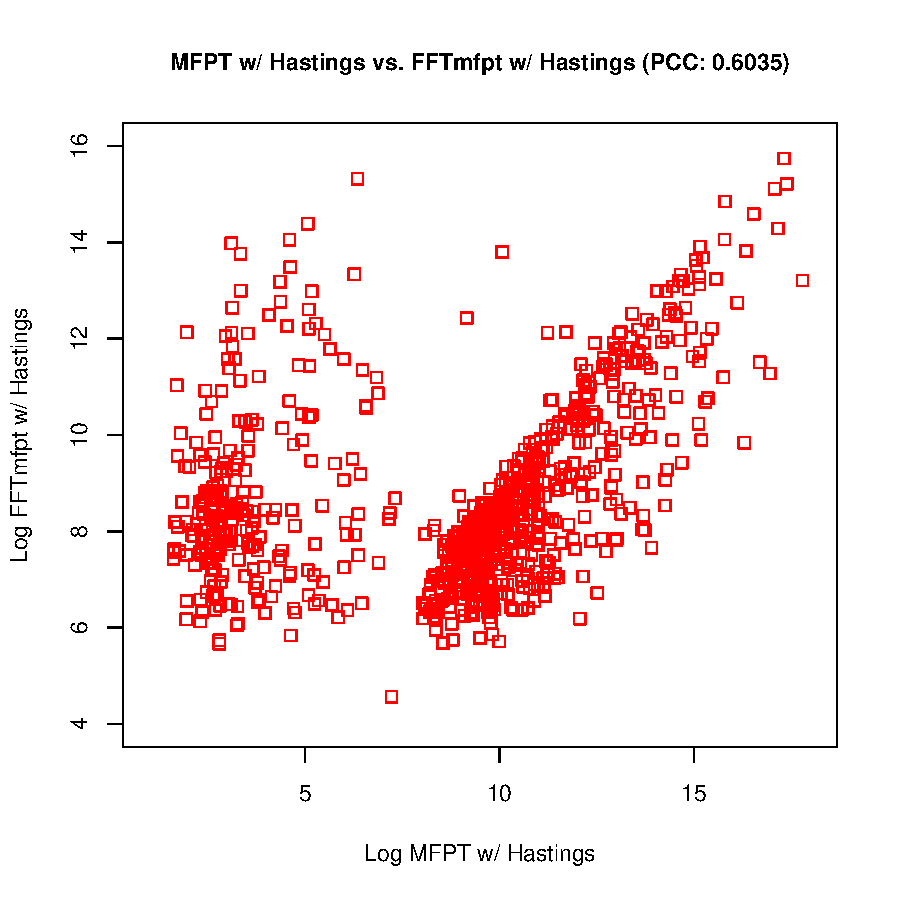
\includegraphics[width=0.45\textwidth]{Figures/Hermes/rnaMfptHastingsFftMfptHastings.pdf}
\caption[Scatter plots of the natural logarithm of times from \rnamfpt
versus \msresp{Kinfold} {\em (Left)} and for \rnamfpt versus \msresp{FFTmfpt} {\em (Right)}]
{Scatter plots of the natural logarithm of times from \rnamfpt
versus \msresp{Kinfold} {\em (Left)} and for \rnamfpt versus \msresp{FFTmfpt} {\em (Right)}.}
\label{fig:hermes:scatterplotRnaMfptHastingsVsKinfoldAndFftMfpt}
\end{figure}

\begin{figure}[!ht]
\centering
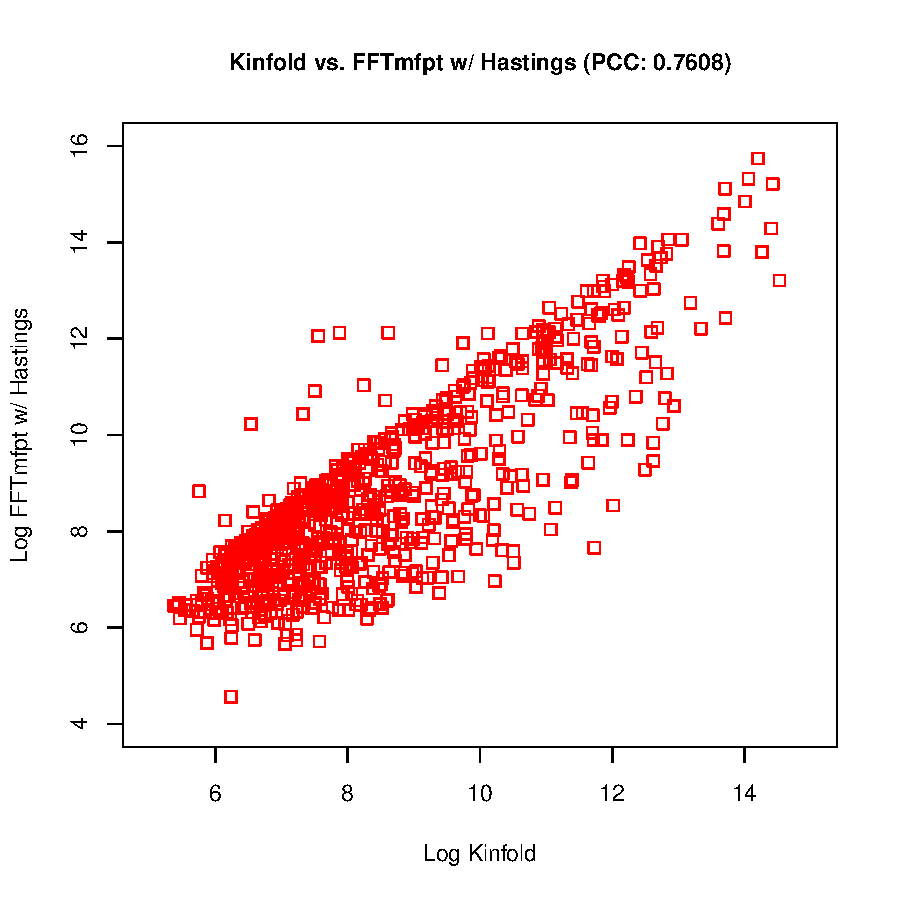
\includegraphics[width=0.45\textwidth]{Figures/Hermes/kinfoldFftMfptHastings.pdf}
\quad
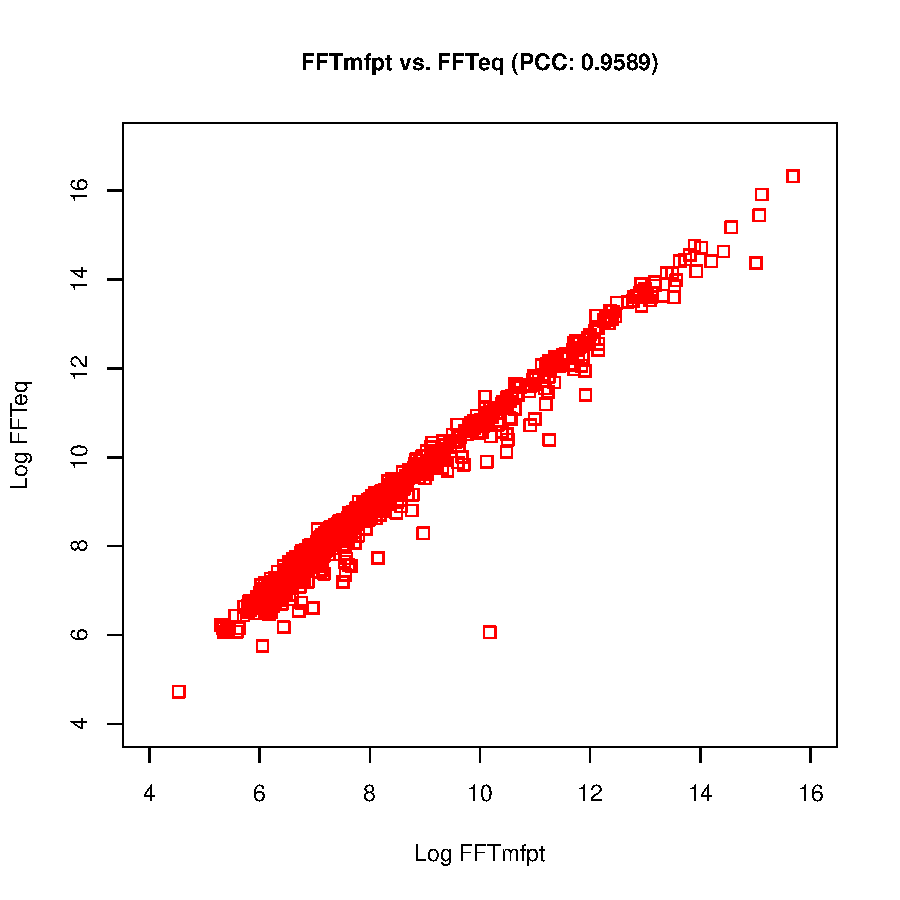
\includegraphics[width=0.45\textwidth]{Figures/Hermes/fftMfptFftEq.pdf}
\caption[Scatter plots of the natural logarithm of times from \kinfold
versus \msresp{FFTmfpt} {\em (Left)} and for \fftmfpt versus \msresp{FFTeq}
{\em (Right)}]{Scatter plots of the natural logarithm of times from \kinfold
versus \msresp{FFTmfpt} {\em (Left)} and for \fftmfpt versus \msresp{FFTeq}
{\em (Right)}.}
\label{fig:hermes:scatterplotFftMfptVsKinfoldAndFftEq}
\end{figure}

\begin{landscape}
\begin{table}[!ht]
\centering
\begin{tabularx}{\linewidth}{c *{8}{L}}
  \toprule
  \small{Hastings (Yes\textbackslash No)} & \small{\rnamfpt} & \small{\rnaeq} & \small{\kinfold} & \small{\fftmfpt} & \small{\rnatwofold} & \small{\fftbor} & \small{\barrierseq} & \small{\ffteq} \\
  \cmidrule(l){2-9}
  \small{\rnamfpt}   & $1$      & $0.5683$ & $0.7945$ & $0.5060$ & $0.5110$ & $0.5204$ & $0.5280$ & $0.4472$ \\
  \small{\rnaeq}   & $0.5798$ & $1$      & $0.7814$ & $0.7043$ & $0.7025$ & $0.5080$ & $0.5979$ & $0.6820$ \\
  \small{\kinfold}       & $0.7933$ & $0.7507$ & $1$      & $0.7312$ & $0.7358$ & $0.6241$ & $0.6328$ & $0.6445$ \\
  \small{\fftmfpt}       & $0.6035$ & $0.7935$ & $0.7608$ & $1$      & $0.9980$ & $0.5485$ & $0.8614$ & $0.9589$ \\
  \small{\rnatwofold}     & $0.6076$ & $0.7919$ & $0.7655$ & $0.9983$ & $1$      & $0.5584$ & $0.8538$ & $0.9515$ \\
  \small{\fftbor}        & $0.5416$ & $0.5218$ & $0.6241$ & $0.5748$ & $0.5855$ & $1$      & $0.3450$ & $0.4229$ \\
  \small{\barrierseq} & $0.6346$ & $0.6578$ & $0.6328$ & $0.8310$ & $0.8217$ & $0.3450$ & $1$      & $0.9149$ \\
  \small{\ffteq}         & $0.5614$ & $0.7916$ & $0.6966$ & $0.9670$ & $0.9590$ & $0.4757$ & $0.8940$ & $1$      \\
  \bottomrule
 \end{tabularx}
 \caption[Table of Pearson correlation coefficients for various methods to compute or approximate
 RNA secondary structure folding kinetics]{Table of Pearson correlation coefficients for
 various methods to compute or approximate RNA secondary structure folding kinetics.
 Lower [resp. upper] triangular entries are with [resp. without] the Hastings correction
 for Markov chain probability matrices. The methods are: \rnamfpt (\mfpt, computed by matrix
 inversion for the Markov chain consisting of all secondary structures, with move allowed between
 structures differing by one base pair), \rnaeq (\eqt, computed by spectral decomposition of a
 rate matrix comprising all secondary structures to compute population fraction $P(t)$ at time $t$),
 \kinfold (an implementation of Gillespie's Algorithm to approximate refolding pathways using an
 event-based Monte Carlo simulation), \fftmfpt (\mfpt for Markov chain consisting of `grid point'
 states $(x,y)$ with probability $P(x,y)=\sum_\str \frac{\boltzf{\str}}{\fullZ}$, computed by \ffttwo,
 where the sum is taken over structures having \bpd $x$ to the empty structure and $y$ to the MFE
 structure, \rnatwofold (\mfpt, computed as previously explained, but using \rnatwofold in place
 of \ffttwo to compute $P(x,y)$), \fftbor (\mfpt, computed for the Markov chain consisting of
 states $0,1,\dots,n$, for which $P(x) = \sum_\str \frac{\boltzf{\str}}{\fullZ}$, where the
 sum is taken over all secondary structures whose \bpd is $x$ from the MFE structure), \barrierseq
 (\eqt, computed using spectral decomposition on the Markov process consisting of `grid point'
 states output from \barriers), and \ffteq (\eqt, computed in the same fashion as \barrierseq
 using a Markov process derived from the energy landscape output by \ffttwo).}
\label{table:correlationHermes}
 \end{table}
 \end{landscape}
